%!TEX root = ./template-skripsi.tex
%-------------------------------------------------------------------------------
%                            BAB III
%               		PEMBAHASAN
%-------------------------------------------------------------------------------

\chapter{IMPLEMENTASI PROGRAM}

Sesuai dengan tahapan-tahapan pengembangan perangkat lunak yang tertera pada SDLC, maka penulis melakukan serangkaian kegiatan untuk menunjang pengembangan aplikasi resep masakan berbasis Android ini. Karena menggunakan SDLC Model Spiral, maka penulis akan melakukan beberapa tahapan yaitu identifikasi, desain, konstruksi dan pembangunan, serta evaluasi. Evaluasi akan dibahas pada Bab IV (Uji Coba dan Hasil Percobaan) Adapun alur dari aplikasi yang akan dibuat dijelaskan pada Gambar \ref{alur_app}

\begin{figure}[H]
	\centering
	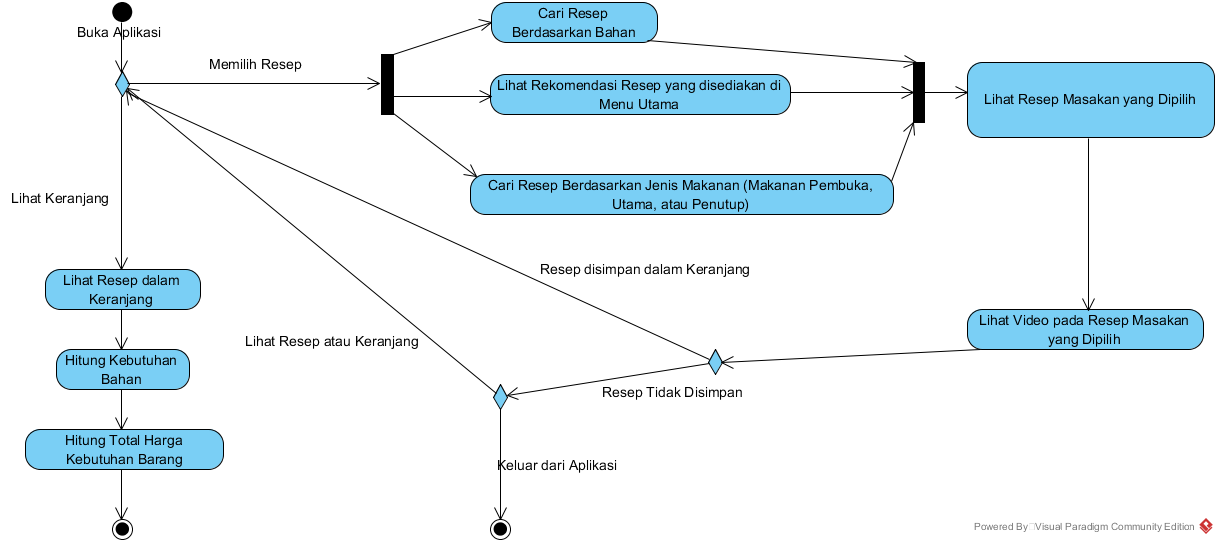
\includegraphics[width=1\textwidth]{gambar/activity_diagram_v2}
	\caption{Alur Kerja Aplikasi}
	\label{alur_app}
\end{figure}


\section{Identifikasi}
	Penulis mengumpulkan beberapa informasi yang dibutuhkan untuk membangun aplikasi ini dengan cara menyebarkan beberapa kuisioner kepada ahli di bidang masakan, baik itu chef, asisten chef, serta pemilik usaha dibidang kuliner untuk mengetahui fitur apa sajakah yang seharusnya ada dalam aplikasi berbasis Android ini. Penulis juga tidak lupa meminta pandangan kepada beberapa kaum awam yang berasal dari berbagai kalangan untuk mengetahui tentang pendapat masyarakat tentang fitur apa saja yang seharusnya terdapat pada aplikasi resep masakan ini. 
	
	Dari 4 responden yang merupakan para ahli, dimana 2 dari 4 responden tersebut adalah chef, satu orang asisten chef, dan seorang pemilik usaha kuliner, fitur menampilkan banyak resep masakan sekaligus merupakan fitur yang paling banyak dipilih dengan nilai 2. Sedangkan fitur lain yang diusulkan penulis seperti menampilkan sebuah resep makanan, menyimpan beberapa resep masakan sekaligus kedalam sebuah troli untuk dibuat dalam jangka waktu tertentu, menghitung total kebutuhan bahan untuk dua resep atau lebih sekaligus, serta menghitung total harga yang dibutuhkan untuk membeli bahan-bahan masakan mendapatkan masing-masing nilai 1.
	
	\begin{figure}[H]
		\centering
		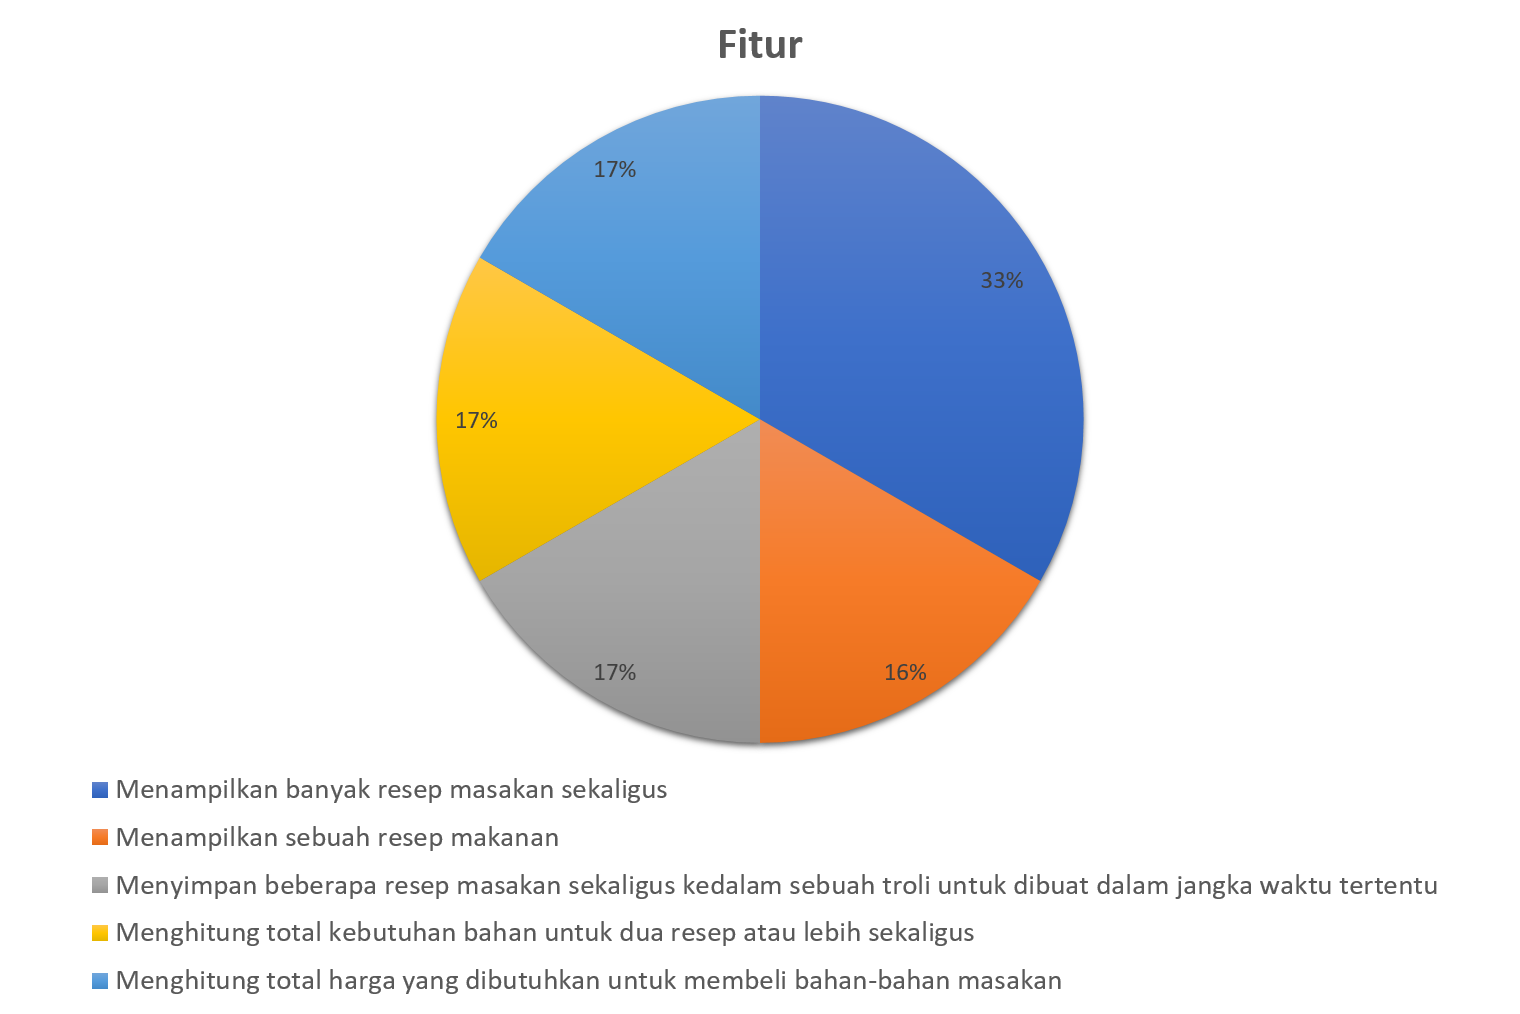
\includegraphics[width=1\textwidth]{gambar/pie/kuisioner_ahli}
		\caption{\textit{Pie Chart} Hasil Kuisioner Ahli}
	\end{figure}
	
	Untuk responden yang berasal dari kaum awam yang berjumlah 9 orang, dimana 2 dari 9 orang responden berprofesi sebagai guru, satu orang berprofesi sebagai ibu rumah tangga, sedangkan sisanya adalah seorang karyawan swasta, fitur menampilkan banyak resep masakan sekaligus merupakan fitur yang paling banyak dipilih dengan nilai 7. Sementara fitur menghitung total kebutuhan bahan untuk dua resep atau lebih sekaligus berada pada peringkat 2 dengan nilai 3. Sedangkan fitur lain yang diusulkan penulis seperti menampilkan sebuah resep makanan, menyimpan beberapa resep masakan sekaligus kedalam sebuah troli untuk dibuat dalam jangka waktu tertentu, serta menghitung total harga yang dibutuhkan untuk membeli bahan-bahan masakan mendapatkan masing-masing nilai 2.
	
	\begin{figure}[H]
		\centering
		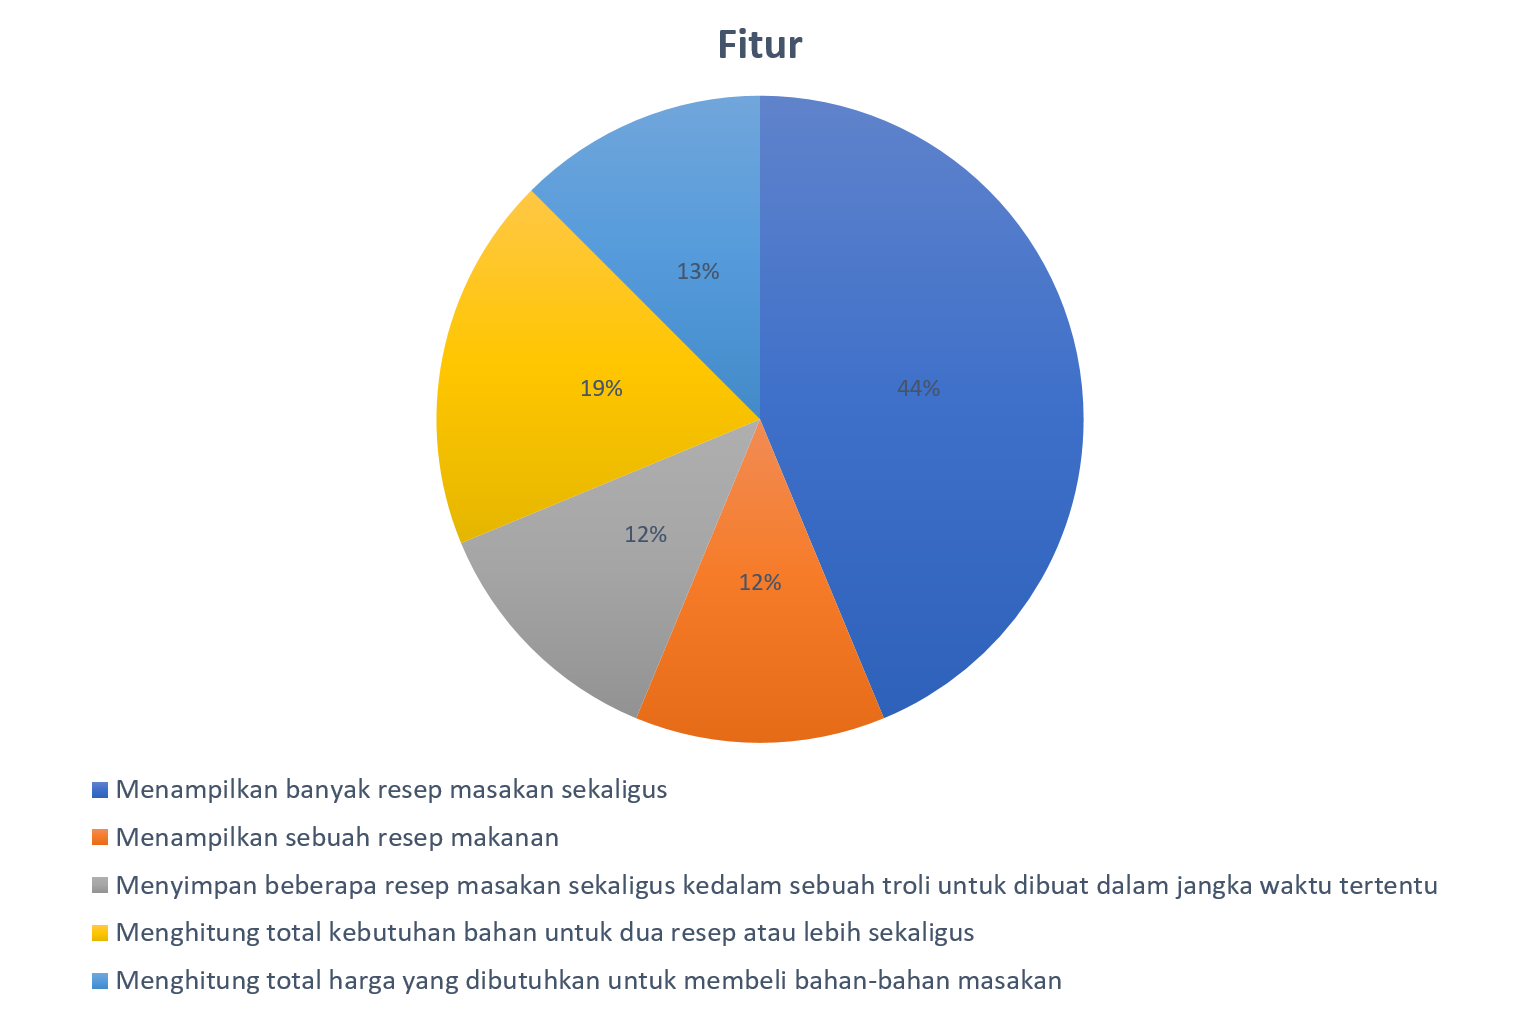
\includegraphics[width=1\textwidth]{gambar/pie/kuisioner_awam}
		\caption{\textit{Pie Chart} Hasil Kuisioner Awam}
	\end{figure}
	
	Masyarakat awam yang menjadi responden pada kuisioner yang telah disebar oleh Penulis menyertakan beberapa pendapat maupun ide tentang fitur apa yang seharusnya dimiliki oleh sebuah sistem aplikasi resep masakan berbasis Android, diantaranya adalah:
	\begin{itemize}
		\item Memberikan deskripsi bahan-bahan makanan yang dibutuhkan juga dan bisa didapatkan dimana
		\item Dalam sebuah resep akan lebih baik jika ada detail resep ini untuk berapa porsi, sehingga orang awam dapat mengetahui berapa takaran bahan-bahan masakan yang akan digunakan untuk porsi tertentu
		\item Menampilkan video tutorial masak, dan alternatif bahan masakan (bahan masakan pengganti untuk alergi misalnya)
		\item Aplikasi disertai video pembuatan masakan dan resepnya.	
	\end{itemize}
	
	Sedangkan dari usulan maupun ide yang datang dari para professional atau ahli di bidang ini adalah sebagai berikut:
	\begin{itemize}		
		\item Memberikan pilihan apa saja yang dapat dimasak dari suatu bahan-bahan tertentu
		\item Mengetahui kapan bahan akan habis
		\item Menampilkan metode memasak yang jelas sesuai dengan standar makanan yang akan dibuat
		\item Informasi jumlah takaran dalam sebuah resep haruslah jelas
		\item Mungkin bisa ditambah dengan foto atau video pembuatannya 
		\item Memberikan tips dan trik 
		\item Memberikan keterangan pada tulisan berbahasa asing untuk menambah pengetahuan. Contohnya \emph{Mise En Place} artinya preparasi
	\end{itemize}

	Melalui data yang telah terhimpun, penulis memutuskan untuk memilih fitur yang banyak dipilih oleh responden, baik ahli maupun kaum awam, untuk diimplemantasikan pada aplikasi yang akan dibuat oleh penulis, yaitu menampilkan banyak resep masakan sekaligus, menghitung total kebutuhan bahan untuk dua resep atau lebih sekaligus, menyimpan beberapa resep masakan sekaligus kedalam sebuah troli untuk dibuat dalam jangka waktu tertentu, serta menghitung total harga yang dibutuhkan untuk membeli bahan-bahan masakan. Sementara, fitur tambahan yang diinisiasi oleh penulis adalah fitur mencari resep berdasarkan bahan masakan yang akan dibuat.
	
\section{Desain}
	Dalam mengembangkan aplikasi ini, penulis mengembangkan desain aplikasi terlebih dahulu, mulai dari desain \emph{Use Case}, \emph{Entity Relationship Diagram} (ERD), \emph{Class Diagram}, serta \emph{Activity Diagram}. Selain itu, penulis juga membuat desain \textit{wireframe} dan \textit{mock-up}. Penulis memutuskan untuk membuat kedua desain tersebut untuk memudahkan pengguna dalam mengeksekusi desain antarmuka dari aplikasi ini. Berdasarkan pengalaman penulis dalam mengikuti program Praktek Kerja Lapangan pada PT Kompas Media Nusantara (Harian Kompas), dimana penulis berperan sebagai \textit{Front-End Developer}, perbedaan dari \textit{wireframe} dan \textit{mock-up} sendiri adalah pada tampilannya. Wireframe mengedepankan \textit{User Experience} dari sebuah laman aplikasi, yaitu alur kerja dari laman aplikasi tersebut. Biasanya tampilan yang disuguhkan oleh \textit{wireframe} tidak terlalu menarik dan hanya terlihat seperti kerangka dari tampilan aplikasi tersebut. 
	\begin{figure}[H]
		\centering
		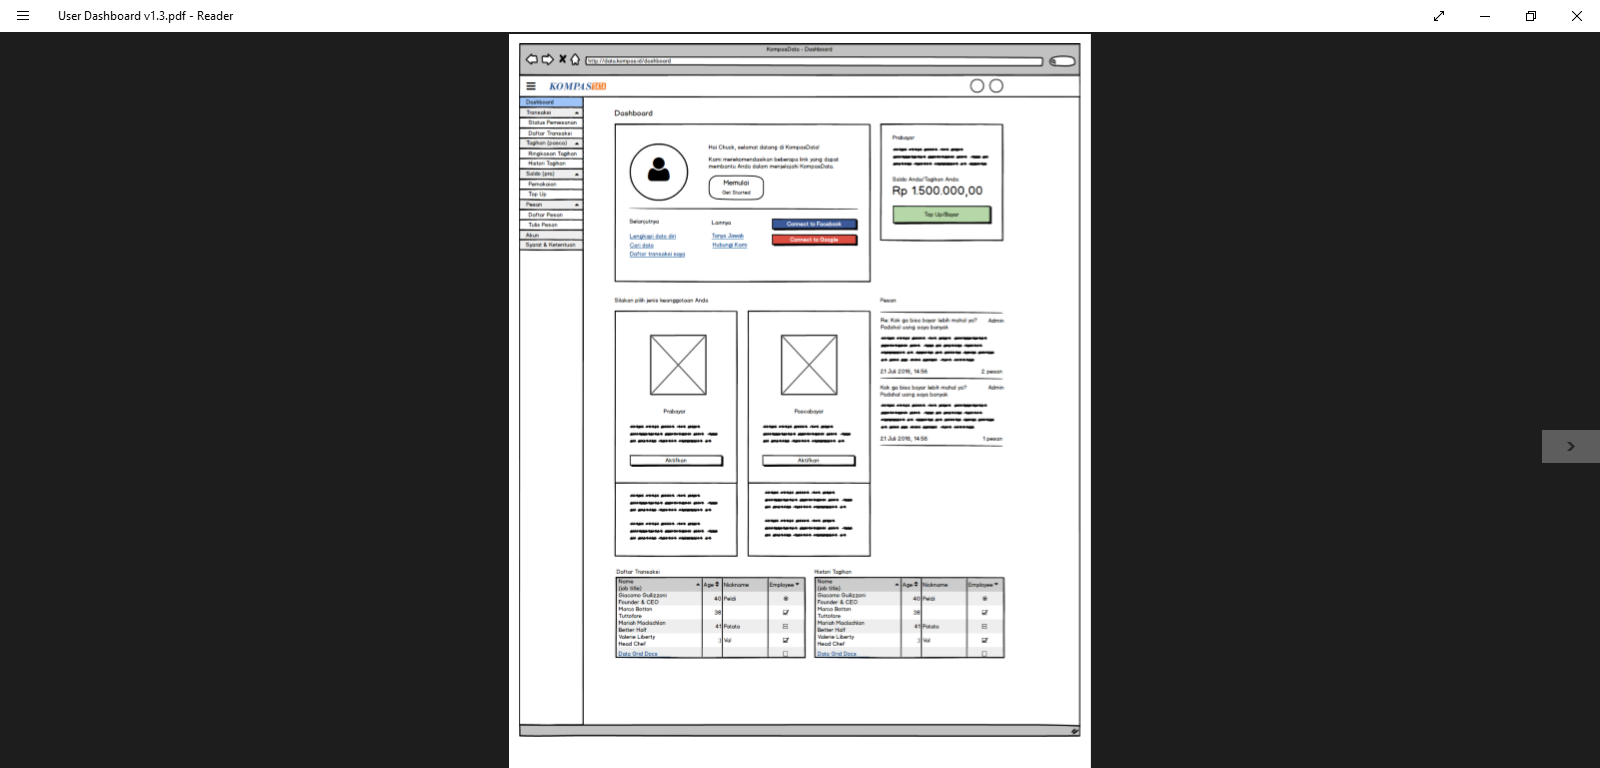
\includegraphics[origin=c,width=0.8\textwidth]{gambar/kompas/wireframe}
		\caption{Contoh \emph{Wireframe}}
		%\label{use case aplikasi}
	\end{figure}
	Sedangkan \textit{mock-up} adalah sebuah rancangan laman antarmuka aplikasi yang bersifat dekoratif dengan dekorasi yang sudah didefinisikan secara jelas oleh pembuatnya. \textit{Mock-up} menonjolkan sisi \textit{User Interface} dari sebuah laman antarmuka aplikasi. Berbeda dengan \textit{wireframe} yang hanya mengedepankan alur kerja dari sebuah laman, \textit{mock-up} adalah pengembangan lebih lanjut dari \textit{wireframe} sehingga sisi estetika dari sebuah rancangan antarmuka aplikasi lebih menonjol. \textit{Mock-up} memudahkan seorang Front-End Developer untuk mengembangkan dan mengeksekusi sebuah laman antarmuka aplikasi.
	\begin{figure}[H]
		\centering
		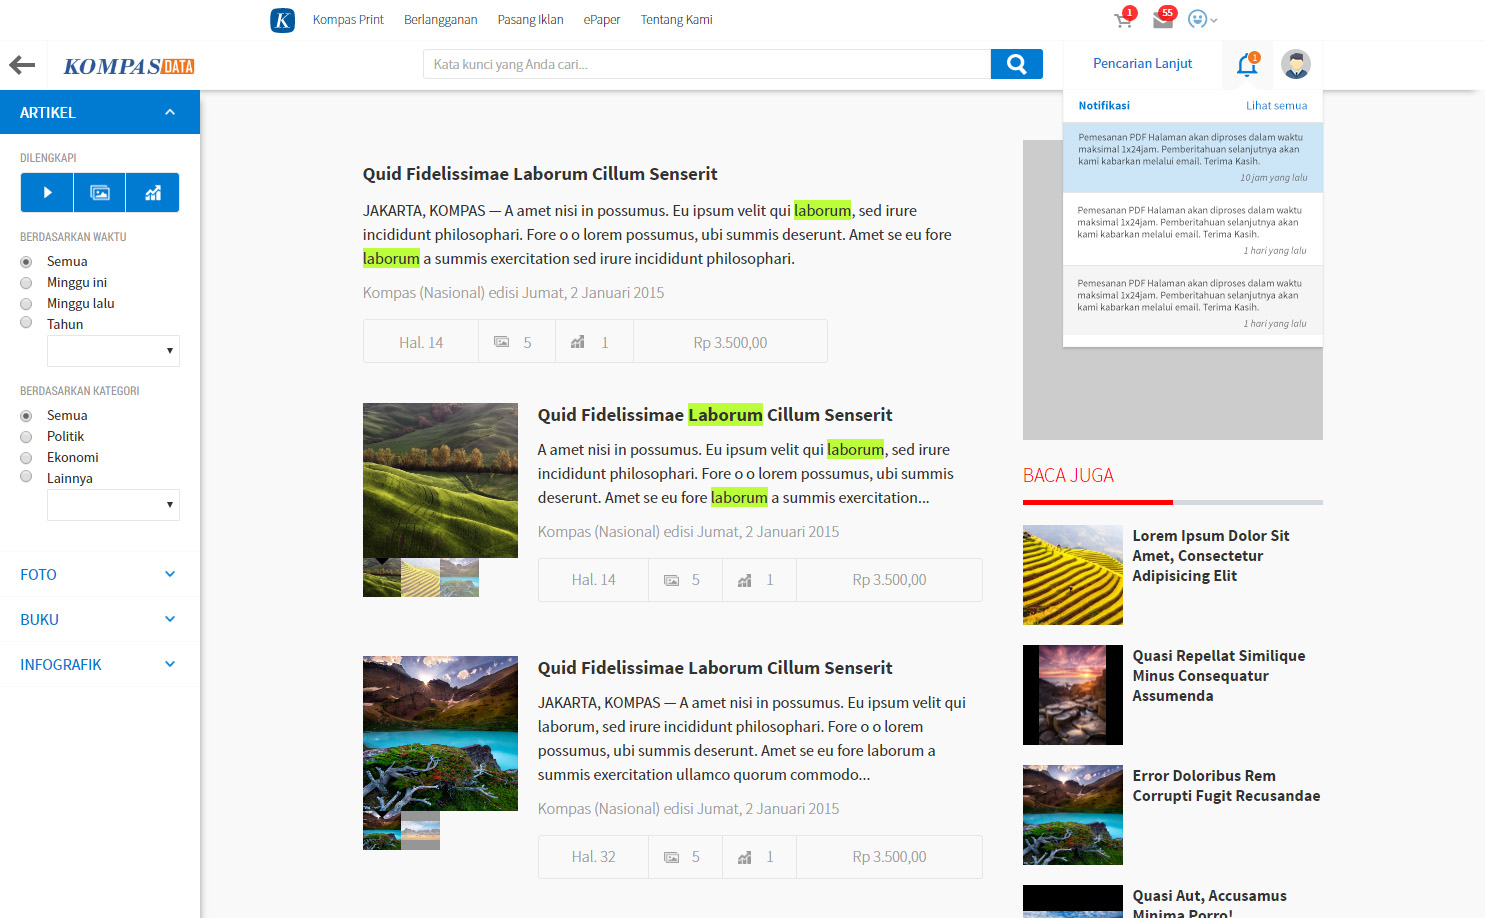
\includegraphics[origin=c,width=0.8\textwidth]{gambar/kompas/mock-up}
		\caption{Contoh \emph{Mock-Up}}
		%\label{use case aplikasi}
	\end{figure}
	 
	\subsection{\emph{Use Case Diagram}}
		\begin{figure}[H]
			\centering
			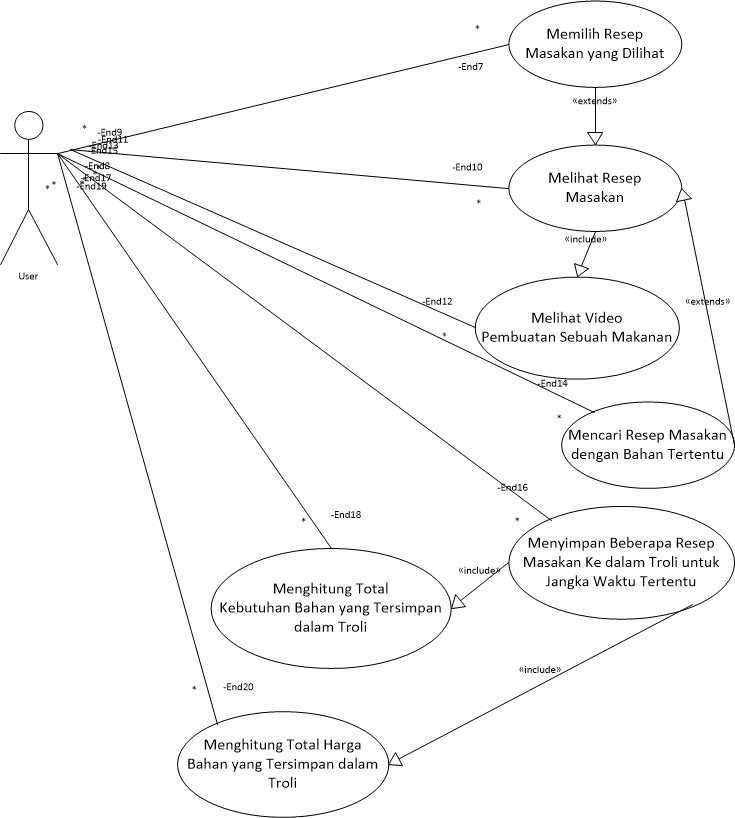
\includegraphics[origin=c,width=0.8\textwidth]{gambar/use-case/use_case_v2}
			%\caption{\emph{Use Case Diagram}}
			%\label{use case aplikasi}
		\end{figure}
		\textit{Use Case Diagram} tersebut menunjukkan bagaimana pengguna aplikasi (\textit{user}) berinteraksi dengan aplikasi yang dikembangkan oleh peneliti. Dalam \textit{use case} tersebut dijelaskan bahwa \textit{user} dapat memilih resep masakan yang ingin dilihat pada menu utama untuk kemudian melihat resep masakan sekaligus melihat video cara membuat makanan yang terdapat dalam resep tersebut. Selain itu, \textit{user} juga dapat mencari resep masakan berdasarkan bahan tertentu sesuai dengan keinginan \textit{user}. Setelah dilihat, \textit{user} dapat menyimpan resep masakan tersebut ke dalam Troli, dimana pada aplikasi ini disebut sebagai \textit{Wishlist}. \textit{User} dapat menyimpan sampai 3 resep masakan sekaligus dalam \textit{Wishlist}. Resep yang ada di dalam \textit{wishlist} dapat dihutung total kebutuhan bahannya dan juga dapat menghitung total kebutuhan harga untuk membeli bahan-bahan tersebut.   
	\subsection{\emph{Entity Relationship Diagram}}
		ERD pada aplikasi ini berfungsi untuk menyimpan resep, kategori resep, bahan-bahan yang ada  pada resep, cara memasak, serta harga pada tiap-tiap bahan yang tercantum dalam resep. Untuk itu, penulis membuat beberapa tabel untuk menunjang penyimpanan data dari tiap elemen tersebut. 
		
		\begin{figure}[H]
			\centering
			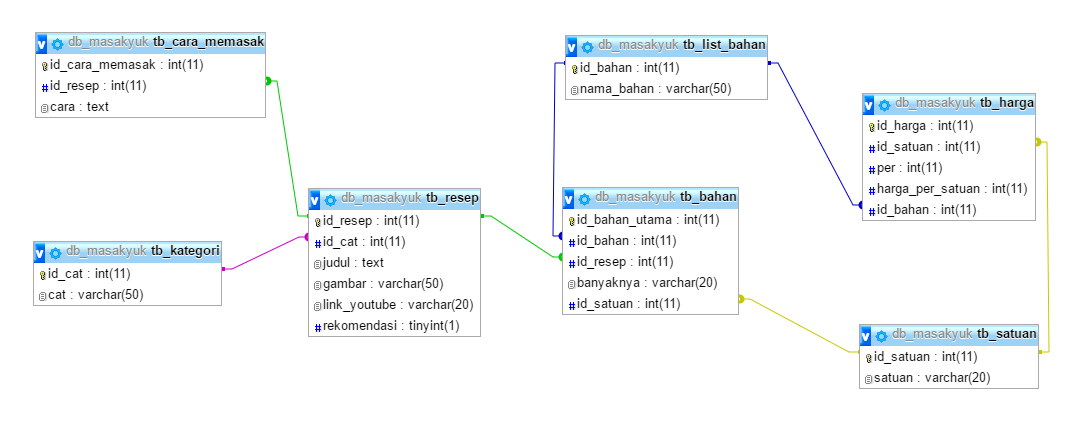
\includegraphics[width=1.1\textwidth]{gambar/erd_terbaru}
			\caption{\emph{Desain ERD Aplikasi yang Dikembangkan Penulis}}
			\label{erd_aplikasi}
			%angle=90,origin=c
		\end{figure}
		
		Penulis menyediakan tabel resep untuk menyimpan data-data yang berhubungan dengan resep. Kemudian, penulis juga menyediakan tabel bahan untuk menyimpan bahan-bahan yang terdapat pada sebuah resep serta tabel list atau daftar bahan untuk menyimpan data bahan-bahan secara umum yang dijadikan sebagai referensi dari tabel bahan. Penulis juga menyediakan tabel harga dan satuan untuk melengkapi tabel bahan. Tabel satuan dibuat karena adanya kemungkinan sebuah bahan dapat memiliki banyak jenis satuan, sedangkan tabel harga dibuat untuk menghitung harga bahan yang tertera dalam tabel bahan dengan kalkulasi yang berbeda bergantung pada satuannya. Selain itu, penulis juga membuat tabel cara memasak untuk menyimpan cara-cara memasak berdasarkan resep yang ada. Terakhir, penulis membuat tabel kategori untuk mengelompokkan rsep berdasarkan jenisnya yaitu Makanan Pembuka, Makanan Utama, dan Makanan Penutup.
		
		Tabel resep berelasi \textit{one-to-many} dengan tabel cara memasak dan tabel bahan karena satu resep dapat memiliki banyak cara memasak dan banyak bahan. Sedangkan tabel kategori berelasi \textit{one-to-many} juga karena satu kategori dapat memiliki banyak resep. Tabel list bahan berelasi \textit{one-to-many} dengan tabel bahan karena bahan yang terdapat pada tabel list bahan dapat dimasukkan lebih dari satu kali pada tabel bahan yang secara langsung menunjang tabel resep. Tabel Satuan berelasi one-to-many dengan tabel harga dan tabel bahan karena tabel harga dapat memiliki banyak satuan serta tabel bahan yang juga sama, yakni dapat memiliki lebih dari satu satuan.   
	\subsection{\emph{Class Diagram}}
		Pada pengembangan aplikasi resep masakan ini, penulis memecah \textit{class diagram} menjadi tiga bagian, yaitu \textit{class diagram} menu utama, \textit{class diagram} detail resep, dan \textit{class diagram wishlist}.
		
		Terdapat dua model yang diakses pada \textit{class diagram} Menu Utama. Resep Model digunakan untuk menyediakan data resep yang diolah pada \textit{controller} Resep Fragment, Rekomendasi Fragment, dan Jenis Fragment. Bahan Model digunakan untuk menyediakan data resep berdasarkan bahan yang dicari oleh \textit{user}.  \textit{Controller} selanjutnya mengalirkan data yang telah diolah kepada \textit{view} yang terdapat pada masing-masing \textit{controller}. Desain class diagram Mennu Utama dapat dilihat pada Gambar \ref{Class Diagram1}.  

		\begin{figure}[H]
			\centering
			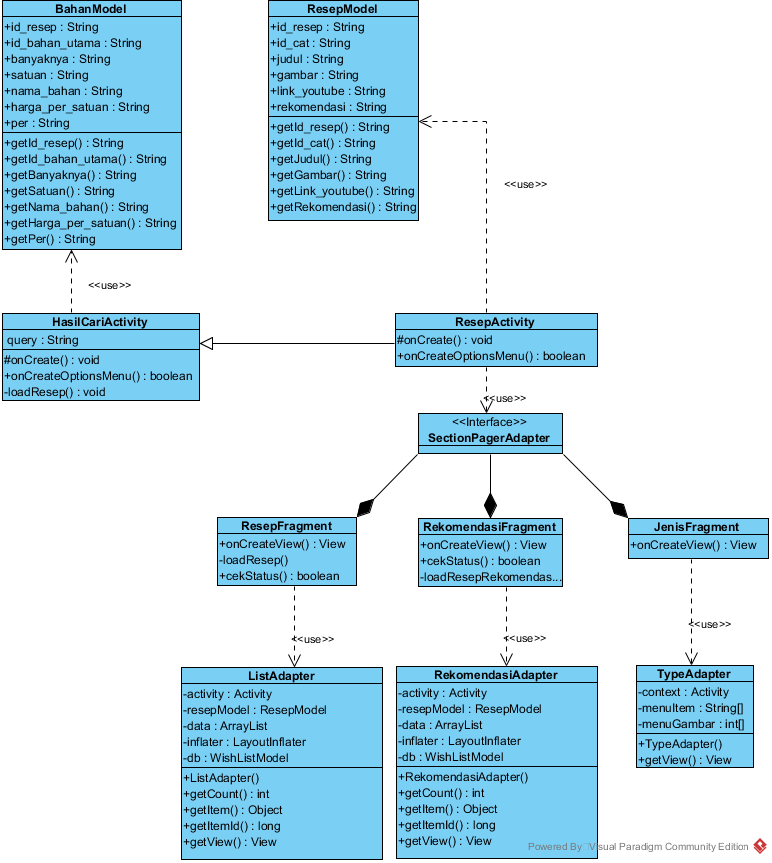
\includegraphics[origin=c,width=1\textwidth]{gambar/class/MenuUtama}
			\caption{\emph{Class Diagram} Menu Utama}
			\label{Class Diagram1}
		\end{figure}
		
		\textit{Class diagram} Detail Resep, yang terdapat pada Gambar \ref{Class Diagram Detail Resep}, memerlukan dua buah model yaitu Bahan Model dan Cara Model. Kedua model tersebut diperlukan untuk menyediakan data bahan yang dibutuhkan serta cara memasak dalam sebuah resep masakan. Data tersebut kemudian diolah dalam \textit{controller} BahanResepFragment dan CaraResepFragment untuk kemudian dialirkan kepada masing-masing \textit{view}
		
		\begin{figure}[H]
			\centering
			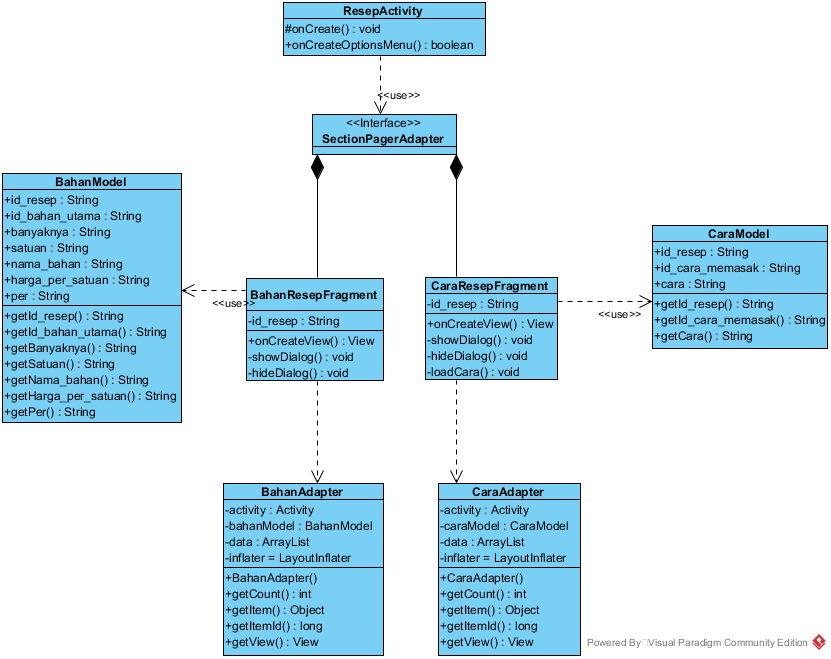
\includegraphics[origin=c,width=1\textwidth]{gambar/class/DetailResep}
			\caption{\emph{Class Diagram} Detail Resep}
			\label{Class Diagram Detail Resep}
		\end{figure}

		Wishlist merupakan \textit{class diagram} terakhir yag dibuat oleh penulis. Terdapat dua model yang digunakan dalam \textit{class diagram} ini yakni Bahan Model dan WishList Model. WishList Model digunakan untuk mengalirkan data resep yang telah disimpan oleh pengguna sebelumnya untuk kemudian dilakukan pencocokan data dengan basis data bahan (Bahan Model). Setelah dicocokkan, pengguna atau \textit{user} dapat melakukan perhitungan total bahan yang dibutuhkan serta melakukan perhitungan total harga bahan yang dibutuhkan oleh pengguna beserta dengan daftar harga tiap bahan yang dibutuhkan. Gambar \textit{class diagram wishlist} dapat dilihat pada Gambar \ref{Class wishlist}.
		
		\begin{figure}[H]
			\centering
			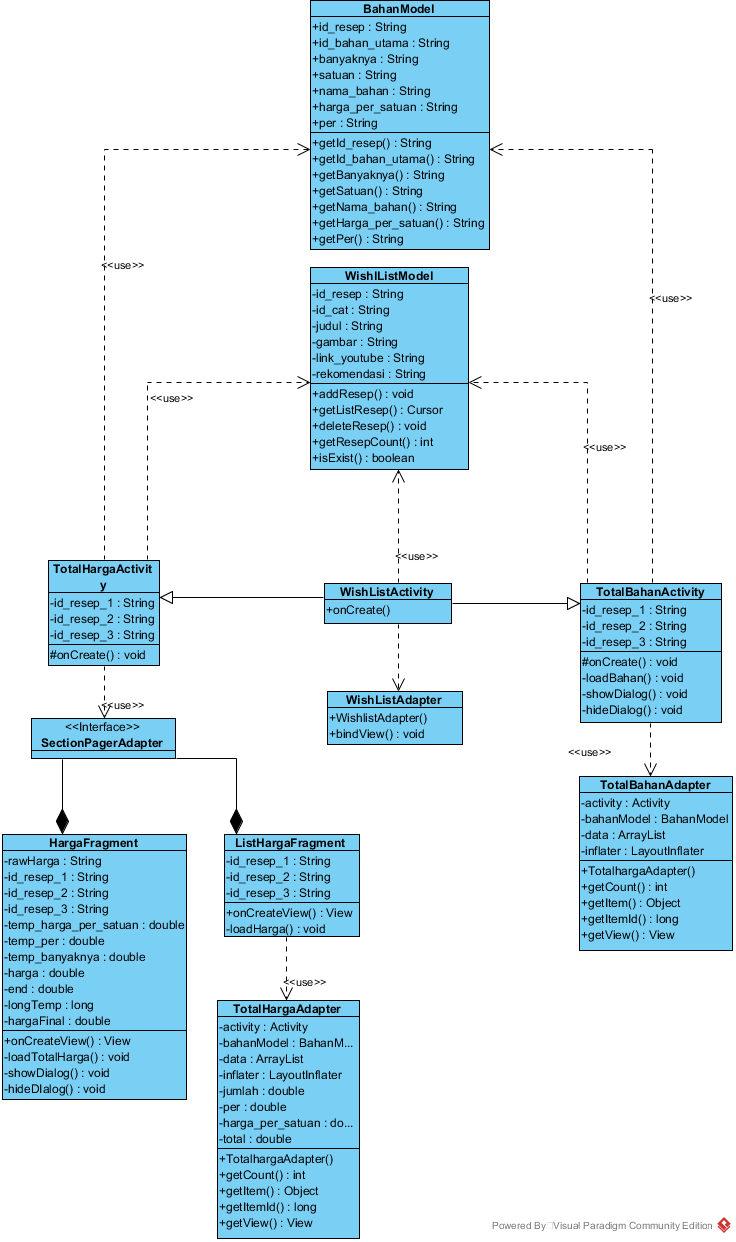
\includegraphics[origin=c,width=0.9\textwidth]{gambar/class/Wishlist}
			\caption{\emph{Class Diagram Wishlist}}
			\label{Class wishlist}
		\end{figure}

	\subsection{\emph{Activity Diagram}}
		Alur kerja aplikasi yang dikembangkan oleh penulis atau peneliti dapat dijelaskan melalui \textit{activity diagram} yang terdapat pada Gambar \ref{Activity Diagram1}
		\begin{figure}[H]
			\centering
			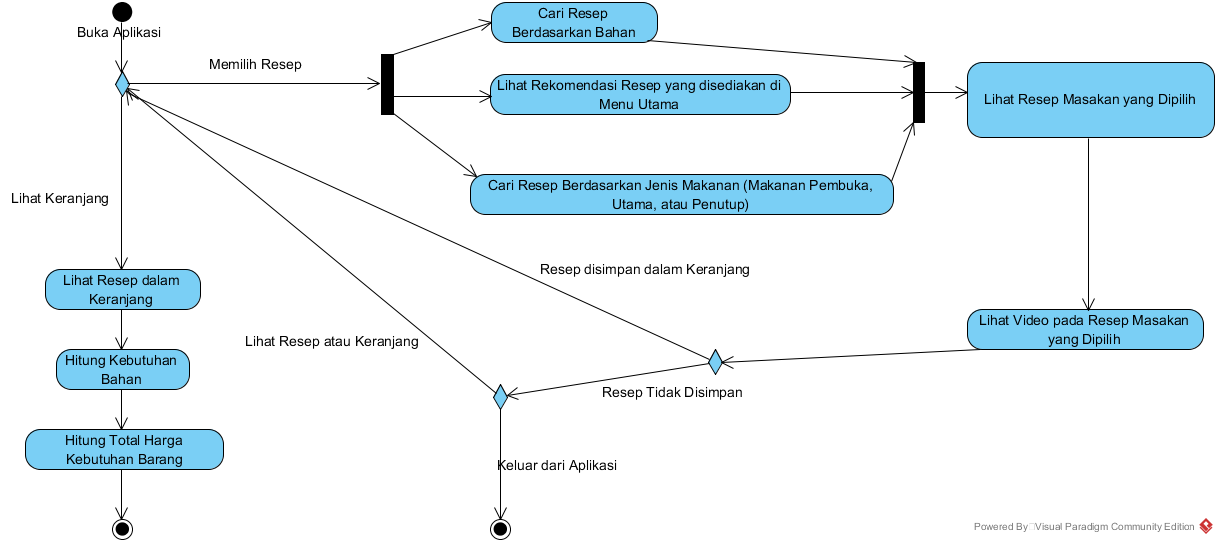
\includegraphics[origin=c,width=1\textwidth]{gambar/activity_diagram_v2}
			\caption{\emph{Activity Diagram dari Aplikasi yang Dibuat Penulis}}
			\label{Activity Diagram1}
		\end{figure}
		 Pada awal membuka aplikasi, pengguna aplikasi dapat memilih resep atau ingin melihat keranjang atau \textit{wishlist} apabila sudah pernah memasukkan resep ke dalam keranjang sebelumnya. Apabila pengguna ingin meilhat resep, maka pengguna dapat memilih resep dengan cara melihat daftar resep, mencari resep berdasarkan bahan, melihat rekomendasi resep yang disediakan, serta mencari resep berdasarkan jenis makanan (makanan pembuka, makanan utama, dan makanan penutup). Setelah itu, pengguna melihat resep yang telah dipilih serta dapat melihat video pembuatannya juga. Apabila resep disimpan kedalam keranjang, maka pengguna dapat kembali memilih resep atau melihat keranjang langsung untuk menghitung kebutuhan bahan serta total harga kebutuhan bahan. Sedangkan apabila resep masakan yang telah dilihat tidak dimasukkan ke dalam keranjang, maka pengguna dapat memilih resep masakan kembali, melihat keranjang yang sudah diisi sebelumnya, atau dapat keluar dari aplikasi.] 
	\subsection{Desain \textit{Wireframe} atau Kerangka Desain}
		\begin{figure}[H]
			\centering
			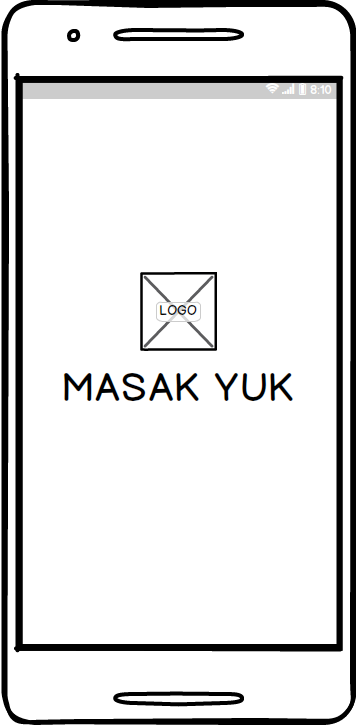
\includegraphics[width=0.25\textwidth]{gambar/wireframe/Splash}
			\caption{Halaman Awal}
			\label{splash}
		\end{figure}
		Desain halaman selamat datang ketika aplikasi pertama kali dimulai ditunjukkan pada Gambar \ref{splash}. Terdapat logo serta gambar latar belakang yang dibuat oleh penulis. Setelah tiga detik, pengguna akan diarahkan kepada laman utama aplikasi yang terdapat pada Gambar \ref{menu_utama} 
		\begin{figure}[H]
			\centering
			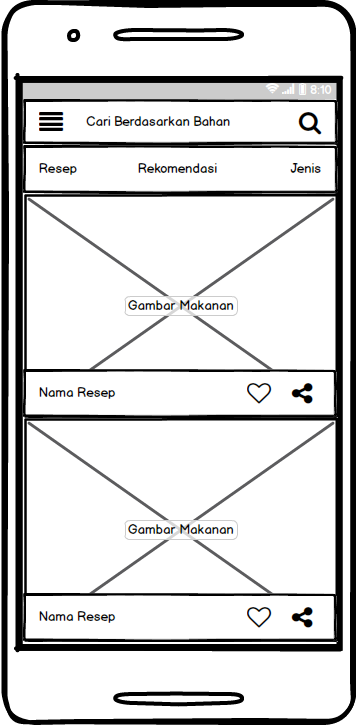
\includegraphics[width=0.25\textwidth]{gambar/wireframe/MenuUtama}
			\caption{Menu Utama}.
			\label{menu_utama} 
		\end{figure}
		Terdapat banyak resep masakan yang dapat dipilih pada laman ini. Pada laman menu utama, apabila pengguna mengusap layar dari rah kiri ke kanan, maka akan muncul menu navigasi seperti pada Gambar \ref{nav}. Pada menu navigasi, pengguna dapat memilih untuk melihat \textit{wishlist}, memberi masukan unuk aplikasi, membagikan aplikasi ke media sosial, dan keluar dari aplikasi
		\begin{figure}[H]
			\centering
			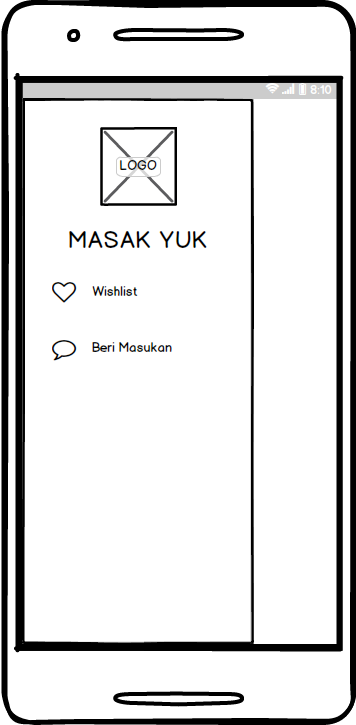
\includegraphics[width=0.25\textwidth]{gambar/wireframe/Drawer}
			\caption{Navigasi}
			\label{nav}
		\end{figure}
		Kembali lagi pada menu utama, apabila pengguna mengusap layar ke kanan atau menekan tab rekomendasi, maka akan muncul resep masakan yang direkomendasikan oleh aplikasi.
		\begin{figure}[H]
			\centering
			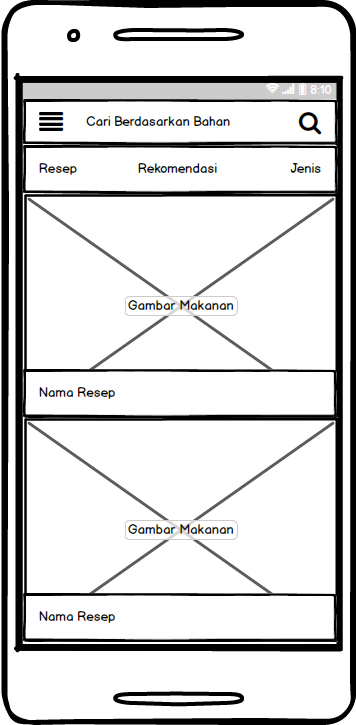
\includegraphics[width=0.25\textwidth]{gambar/wireframe/Rekomendasi}
			\caption{Menu Utama \textit{Tab} Rekomendasi}
		\end{figure}
		\vspace{2cm}
		Pada tab rekomendasi, apabila pengguna mengusap layar ke arah kanan, maka pengguna akan menemukan pilihan penampilan resep berdasarkan jenis makanannya yaitu makanan pembuka, makanan utama, dan makanan penutup.
		\begin{figure}[H]
			\centering
			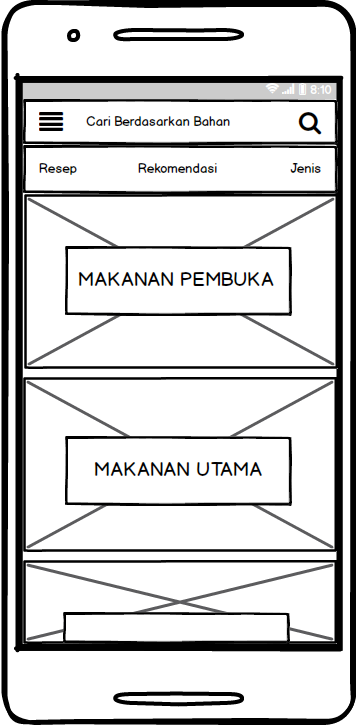
\includegraphics[width=0.25\textwidth]{gambar/wireframe/Jenis}
			\caption{Menu Utama \textit{Tab} Jenis}
		\end{figure}
		Apabila pengguna memilih satu dari resep yang berada pada list yang disediakan dari menu-menu yang telah disebutkan sebelumnya, maka akan muncul laman detail resep yang terdiri dari video, bilah bahan resep serta bilah cara memasak dari resep tersebut
		\begin{figure}[H]
			\centering
			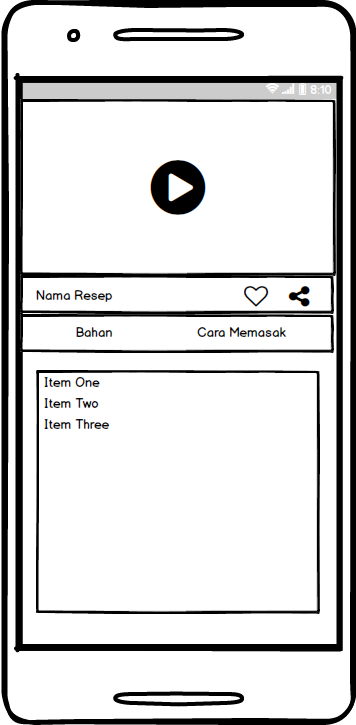
\includegraphics[width=0.25\textwidth]{gambar/wireframe/Resep}
			\caption{Detail Resep}
		\end{figure}
		Pengguna juga dapat melihat \textit{wishlist} dengan memanggil menu navigasi seperti pada Gambar \ref{nav} dan memilih menu \textit{wishlist}. Laman wishlist akan muncul seperti pada Gambar \ref{wire-wish}
		\begin{figure}[H]
			\centering
			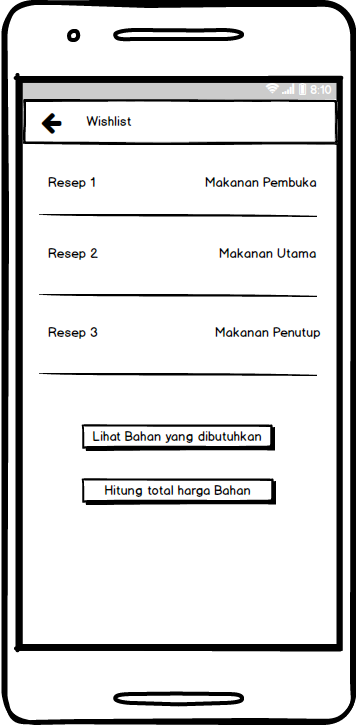
\includegraphics[width=0.25\textwidth]{gambar/wireframe/Wishlist}
			\caption{Keranjang atau \textit{Wishlist}}
			\label{wire-wish}
		\end{figure}
		Pada laman \textit{wishlist}, pengguna dapat menghitung total bahan yang dibutuhkan untuk memasakn berdasarkkan resep yang telah dipilih dan ada pada keranjang
		\begin{figure}[H]
			\centering
			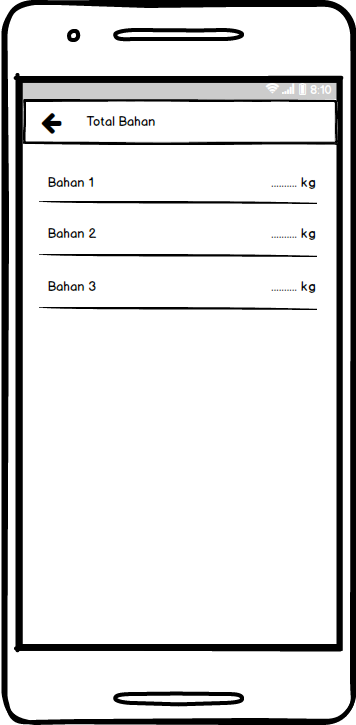
\includegraphics[width=0.25\textwidth]{gambar/wireframe/TotalBahan}
			\caption{Total Bahan}
		\end{figure}
		Selain itu, pada laman \textit{wishlist}, pengguna juga dapat menghitung total harga dari bahan-bahan dari resep yang telah masuk dalam \textit{wishlist}. 
		\begin{figure}[H]
			\centering
			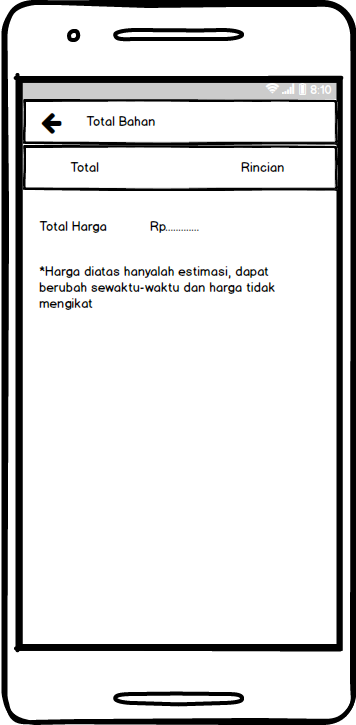
\includegraphics[width=0.25\textwidth]{gambar/wireframe/TotalHarga}
			\caption{Total Harga}
		\end{figure}
	Pengguna juga dapat melihat rincian harga dari tiap bahan yang dibutuhkan oleh resep-resep yang terdapat pada \textit{wishlist}.
		\begin{figure}[H]
			\centering
			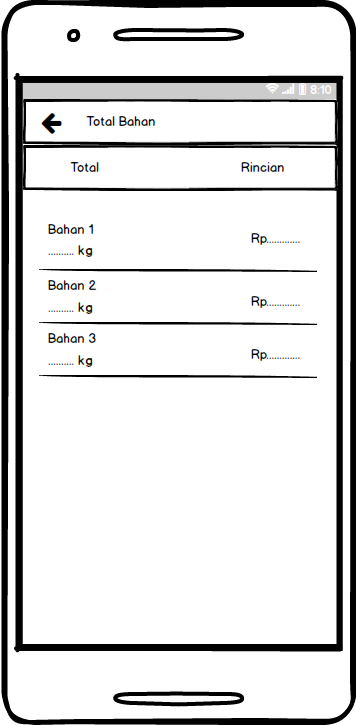
\includegraphics[width=0.25\textwidth]{gambar/wireframe/TotalHargaRincian}
			\caption{Rincian Total Harga}
		\end{figure}
	Kembali ke menu utama, pengguna juga dapat melakukan pencarian resep berdasarkan bahan yang dimiliki oleh pengguna.
		\begin{figure}[H]
			\centering
			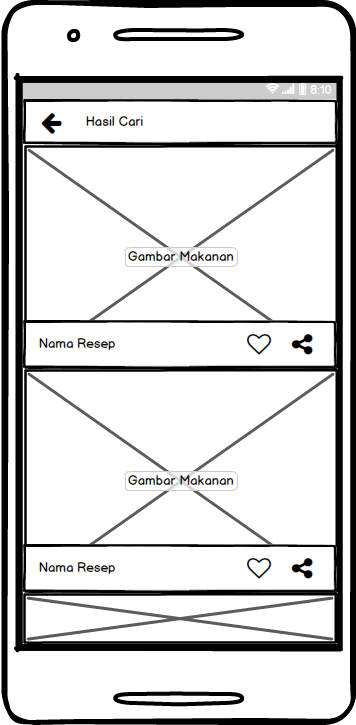
\includegraphics[width=0.25\textwidth]{gambar/wireframe/HasilCari}
			\caption{Hasil Pencarian}
		\end{figure}
	Dan terakhir, desain \textit{wireframe} dari laman beri masukan yang dapat diakses melalui menu navigasi.	
		\begin{figure}[H]
			\centering
			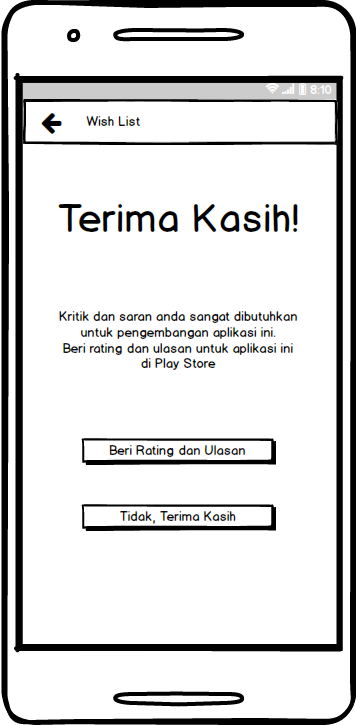
\includegraphics[width=0.25\textwidth]{gambar/wireframe/BeriMasukan}
			\caption{Halaman Beri Masukan}
		\end{figure}
	\subsection{Desain \textit{Mock-Up} atau \textit{User Interface}}
		Setelah membuat wireframe, penulis kemudian langsung mengimplementasikan \textit{wireframe} tersebut ke dalam bentuk \textit{mock-up}. Dalam pengembangannya, \textit{mock-up} langsung dibuat dengan menggunakan xml sehingga mempercepat penulis dalam mengembangkan aplikasi resep masakan ini karena desain dari aplikasi tersebut sudah dikembangkan sekaligus dengan \textit{mock-up}. Selanjutnya penulis hanya perlu mengimplementasikan sistem \textit{Back-End} yang bekerja pada aplikasi resep masakan ini. Pengembangan \textit{mock-up} dapat dilihat pada Gambar \ref{mock-welcome} sampai Gambar \ref{mock-feedback}. Urutan pengembangan \textit{mock-up} sesuai dengan urutan pengembangan \textit{wireframe}.
		\begin{figure}[H]
			\centering
			
\includegraphics[width=0.3\textwidth]{gambar/mock-up/splash}
			\caption{Halaman Awal atau Halaman Selamat Datang}
			\label{mock-welcome}
		\end{figure}
		\begin{figure}[H]
			\centering
			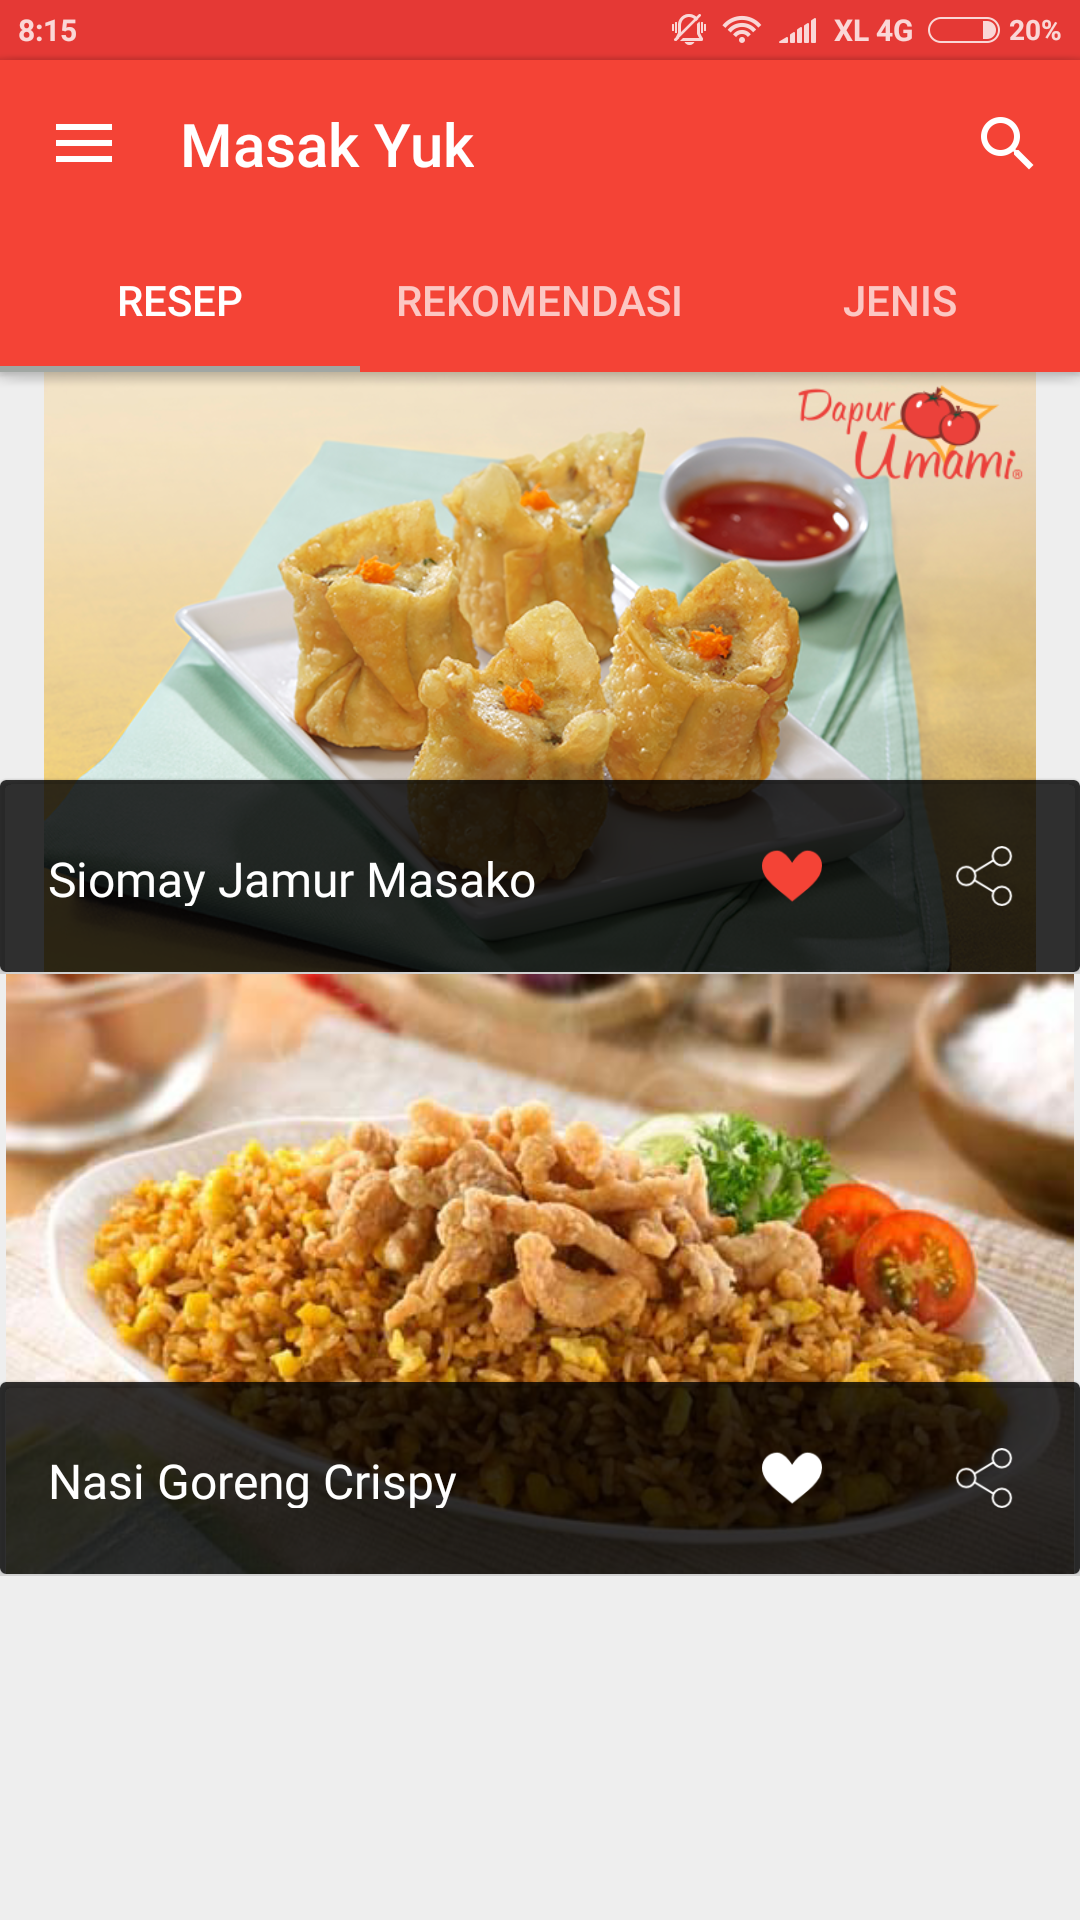
\includegraphics[width=0.3\textwidth]{gambar/mock-up/utama}
			\caption{Halaman Utama}
		\end{figure}
		\begin{figure}[H]
			\centering
			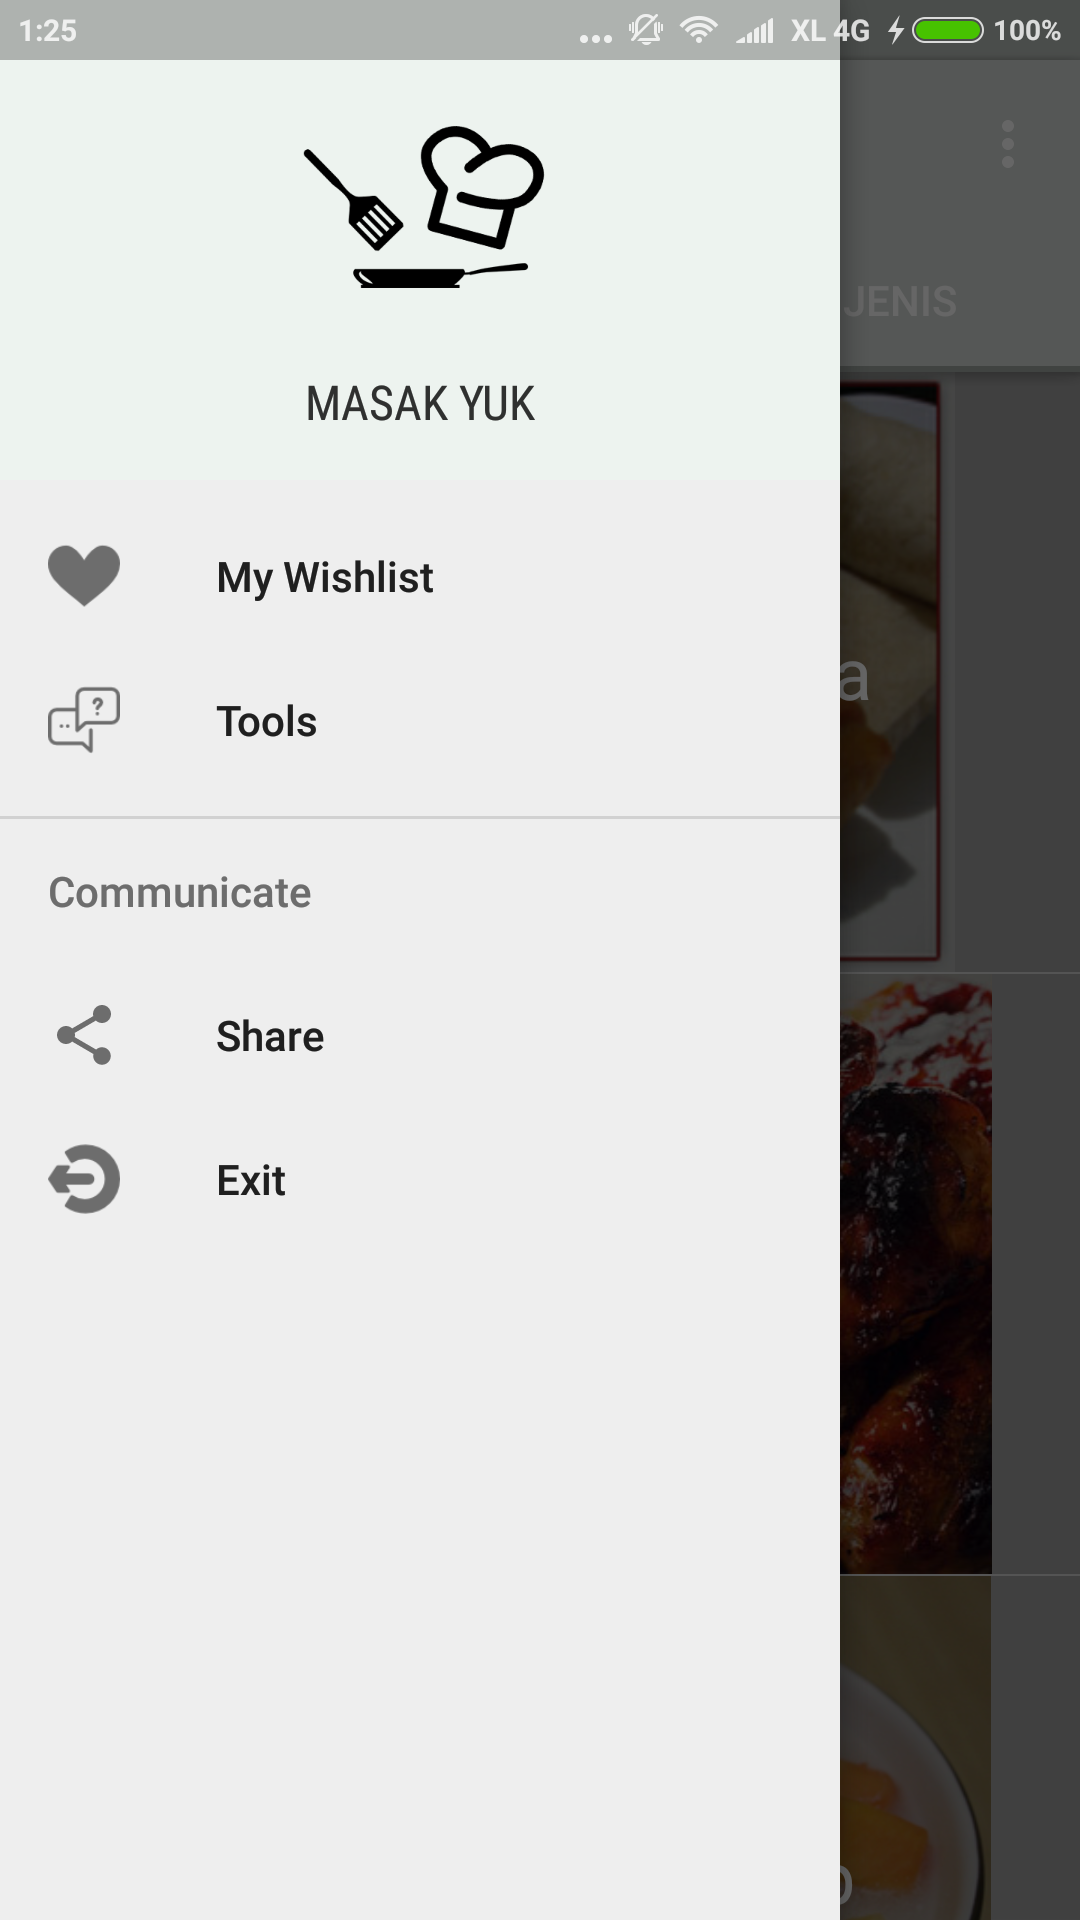
\includegraphics[width=0.3\textwidth]{gambar/mock-up/navigasi}
			\caption{Menu Navigasi}
		\end{figure}			
		\begin{figure}[H]
			\centering
			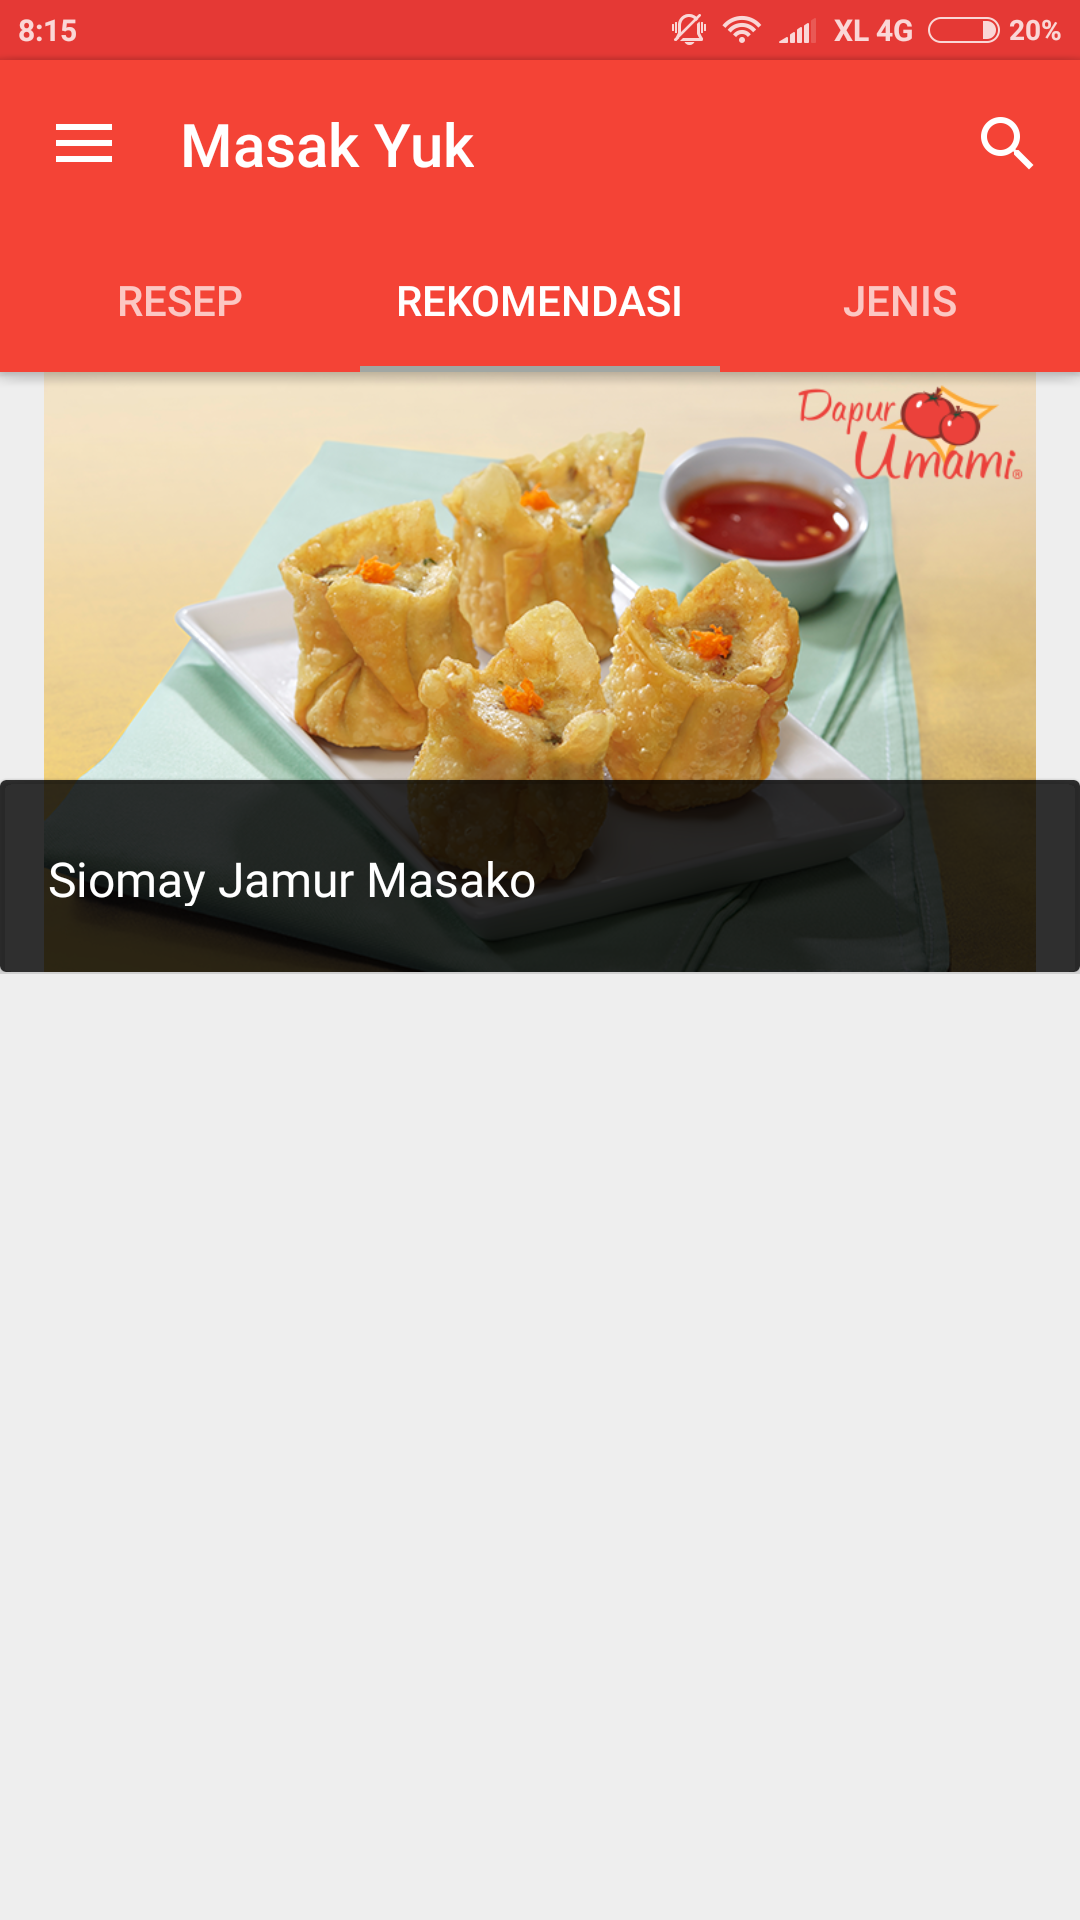
\includegraphics[width=0.3\textwidth]{gambar/mock-up/rekomendasi}
			\caption{Halaman Utama \textit{Tab} Rekomendasi}
		\end{figure}			
		\begin{figure}[H]
			\centering
			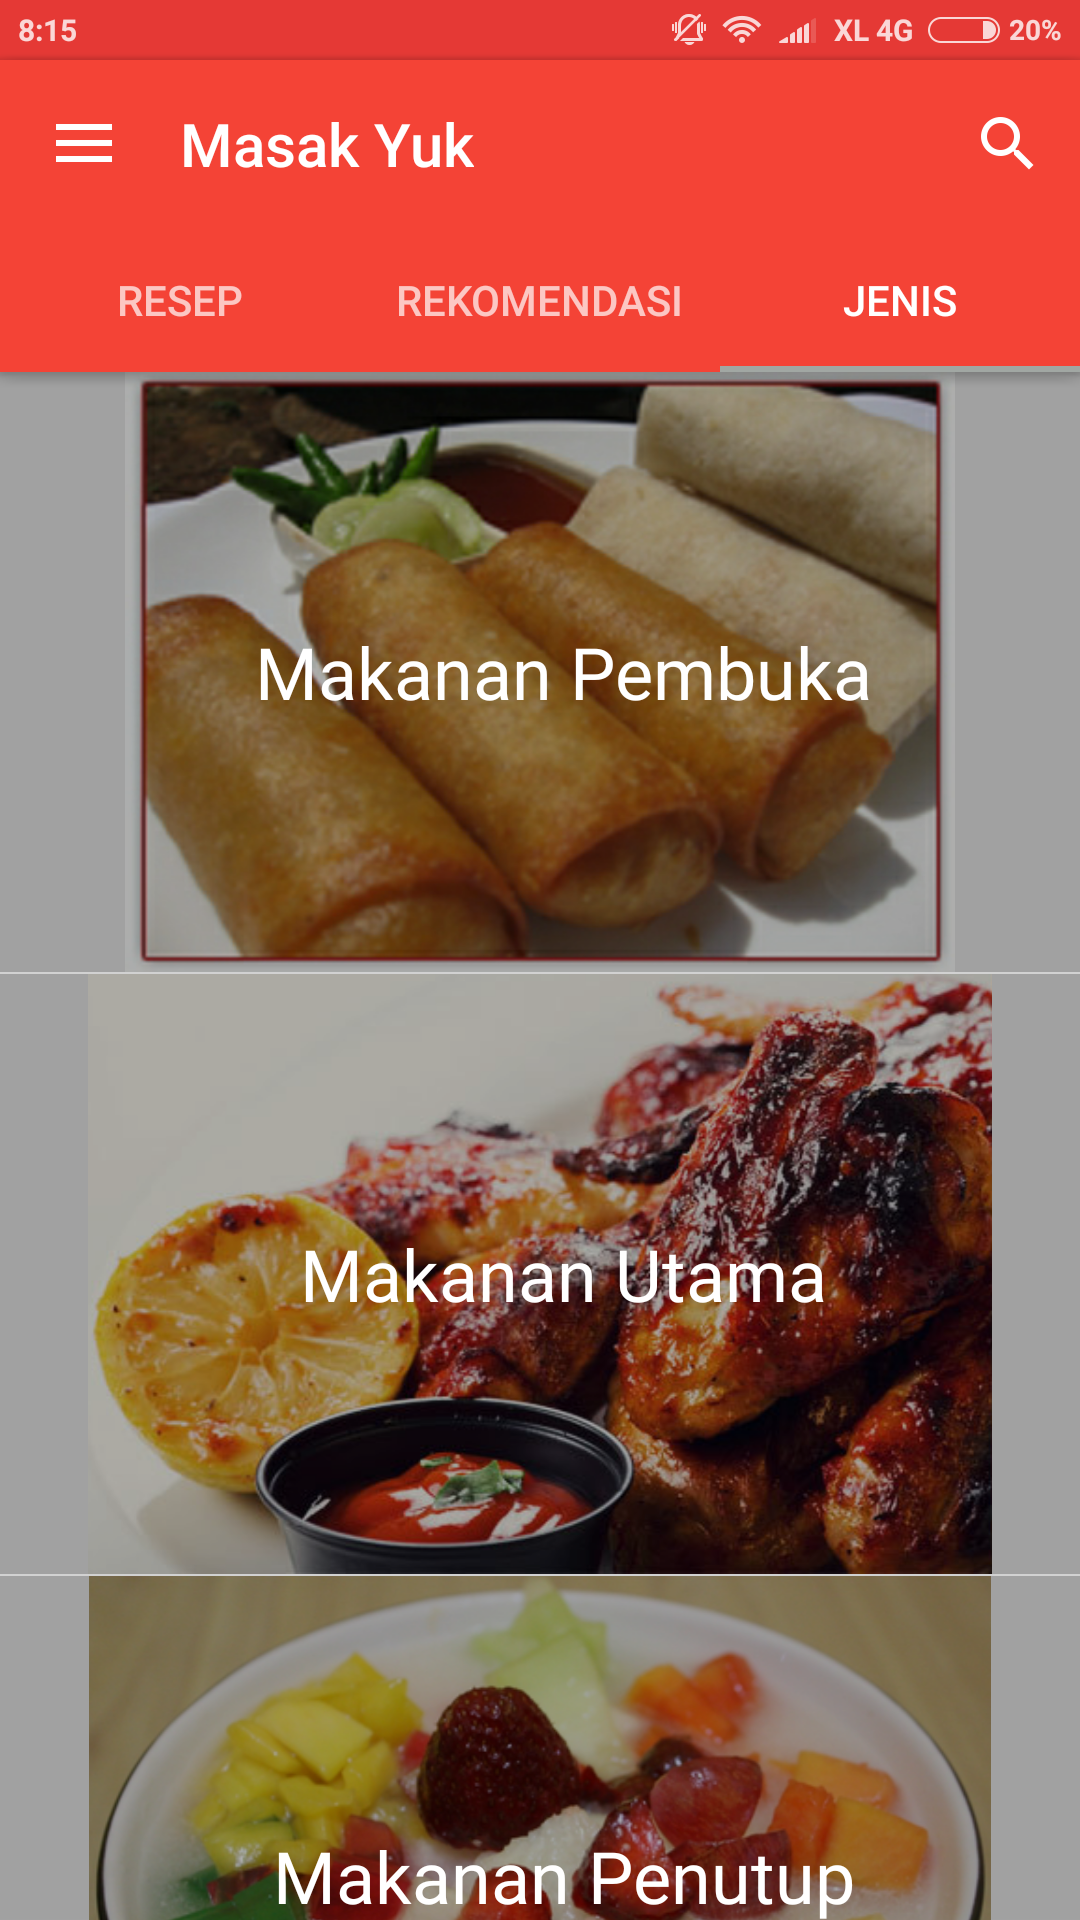
\includegraphics[width=0.3\textwidth]{gambar/mock-up/jenis}
			\caption{Halaman Utama \textit{Tab} Jenis}
		\end{figure}	
		\begin{figure}[H]
			\centering
			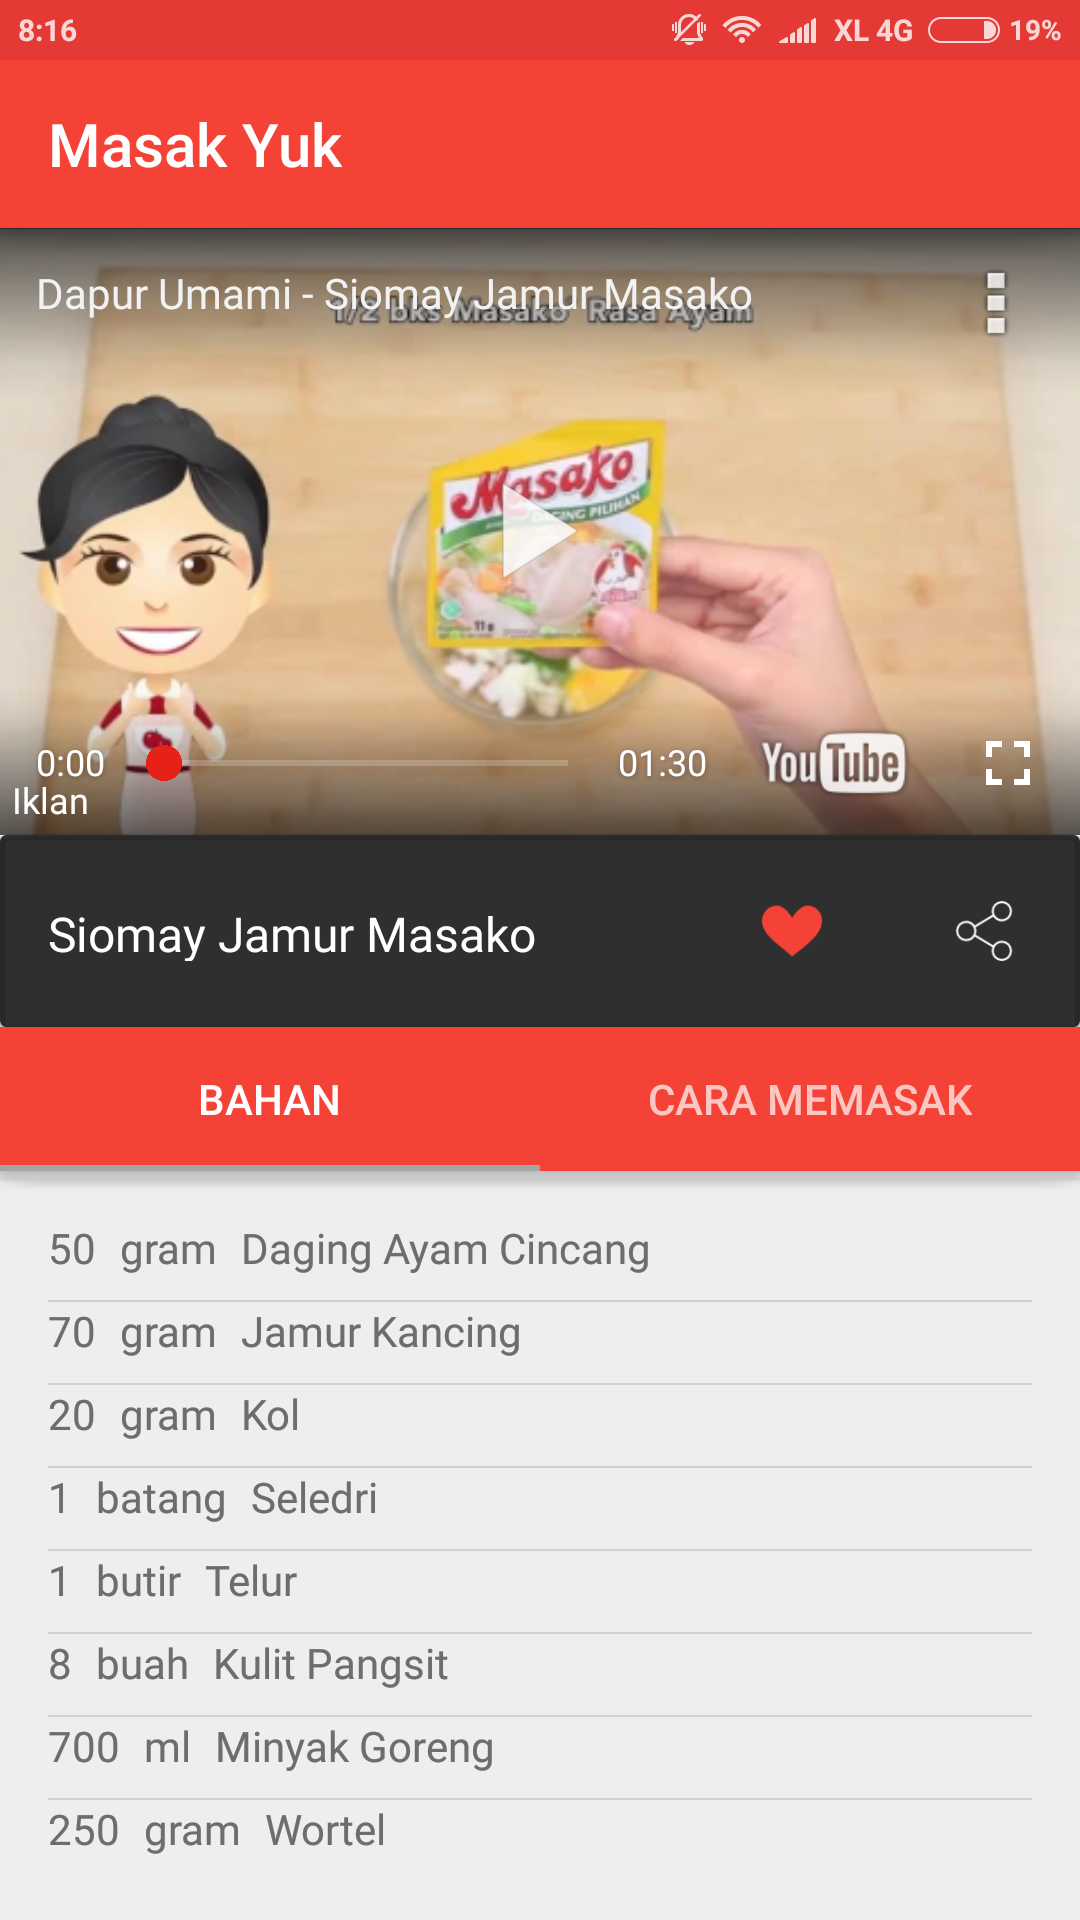
\includegraphics[width=0.3\textwidth]{gambar/mock-up/Detail}
			\caption{Detail Bahan Resep}
			\label{detail_bahan}
		\end{figure}
		\begin{figure}[H]
			\centering
			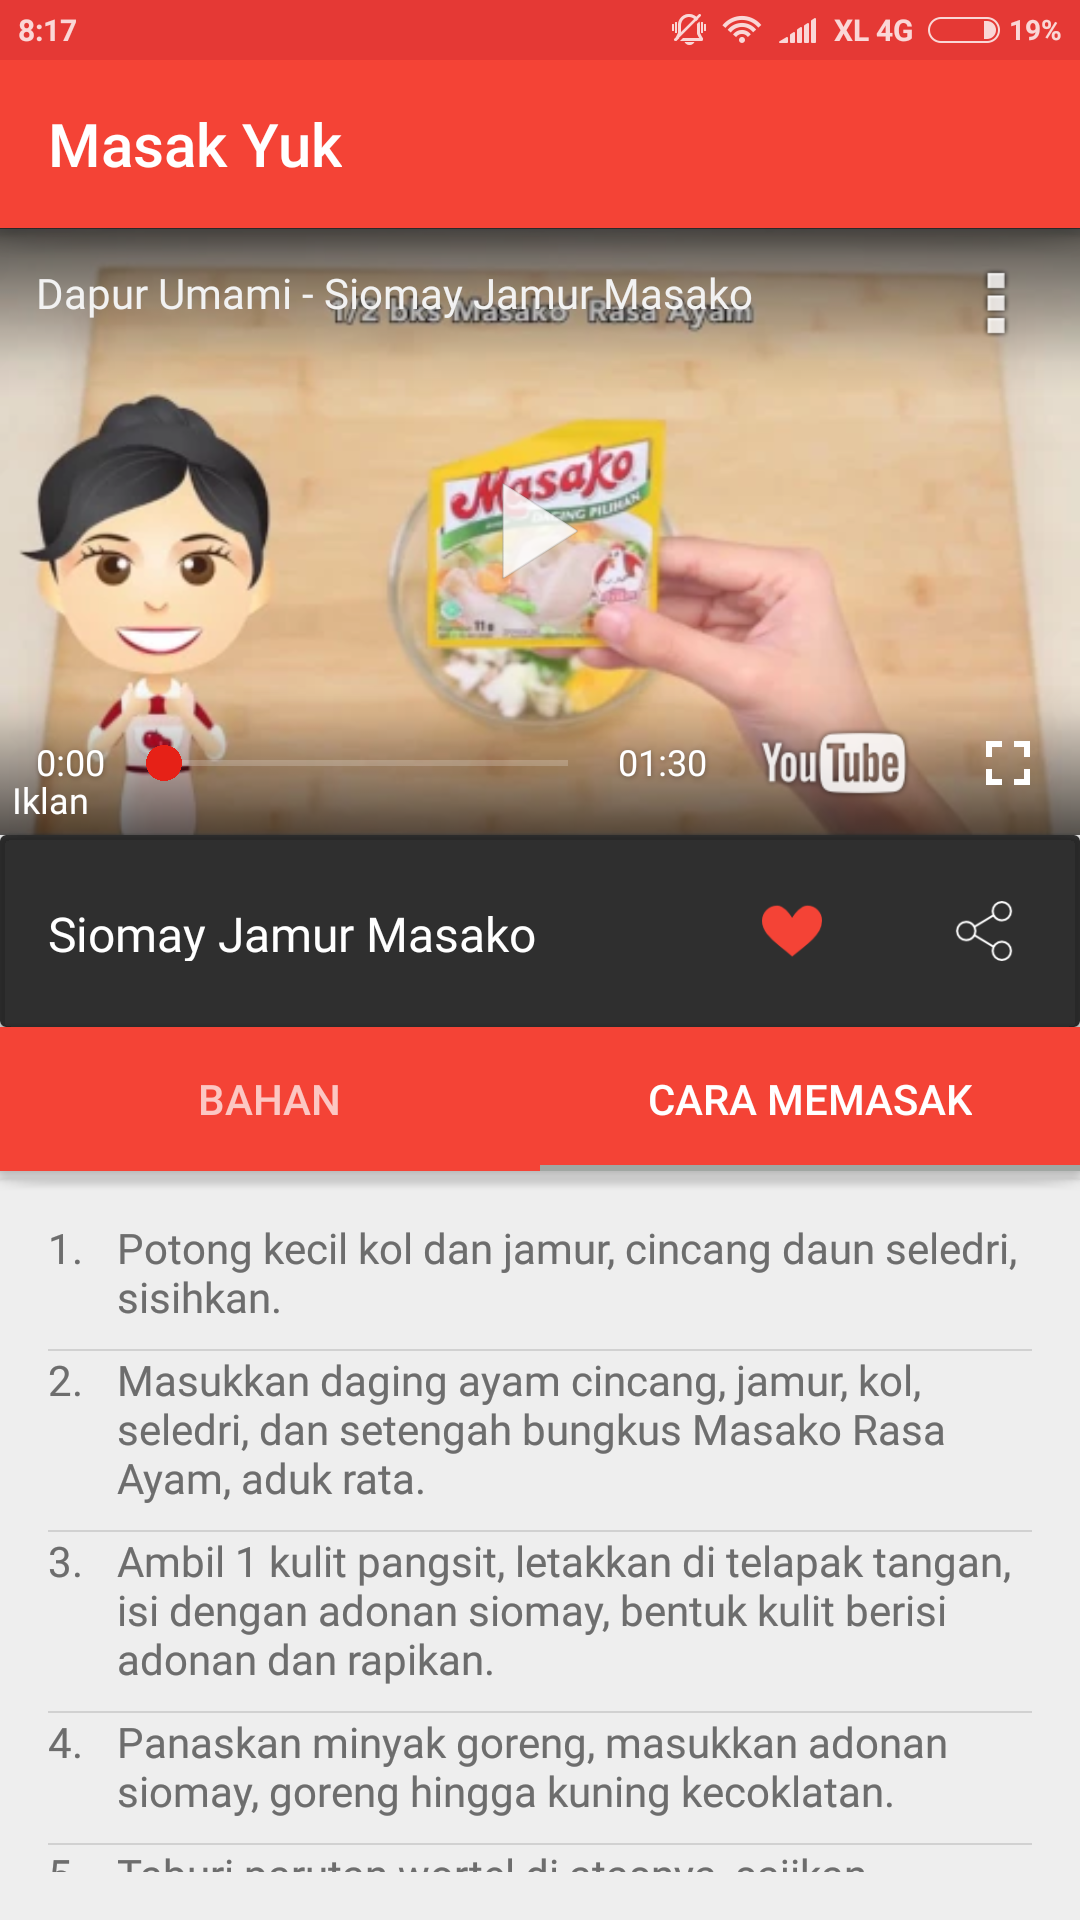
\includegraphics[width=0.3\textwidth]{gambar/mock-up/detail_cara}
			\caption{Detail Cara Memasak}
			\label{detail_cara}
		\end{figure}
		\begin{figure}[H]
			\centering
			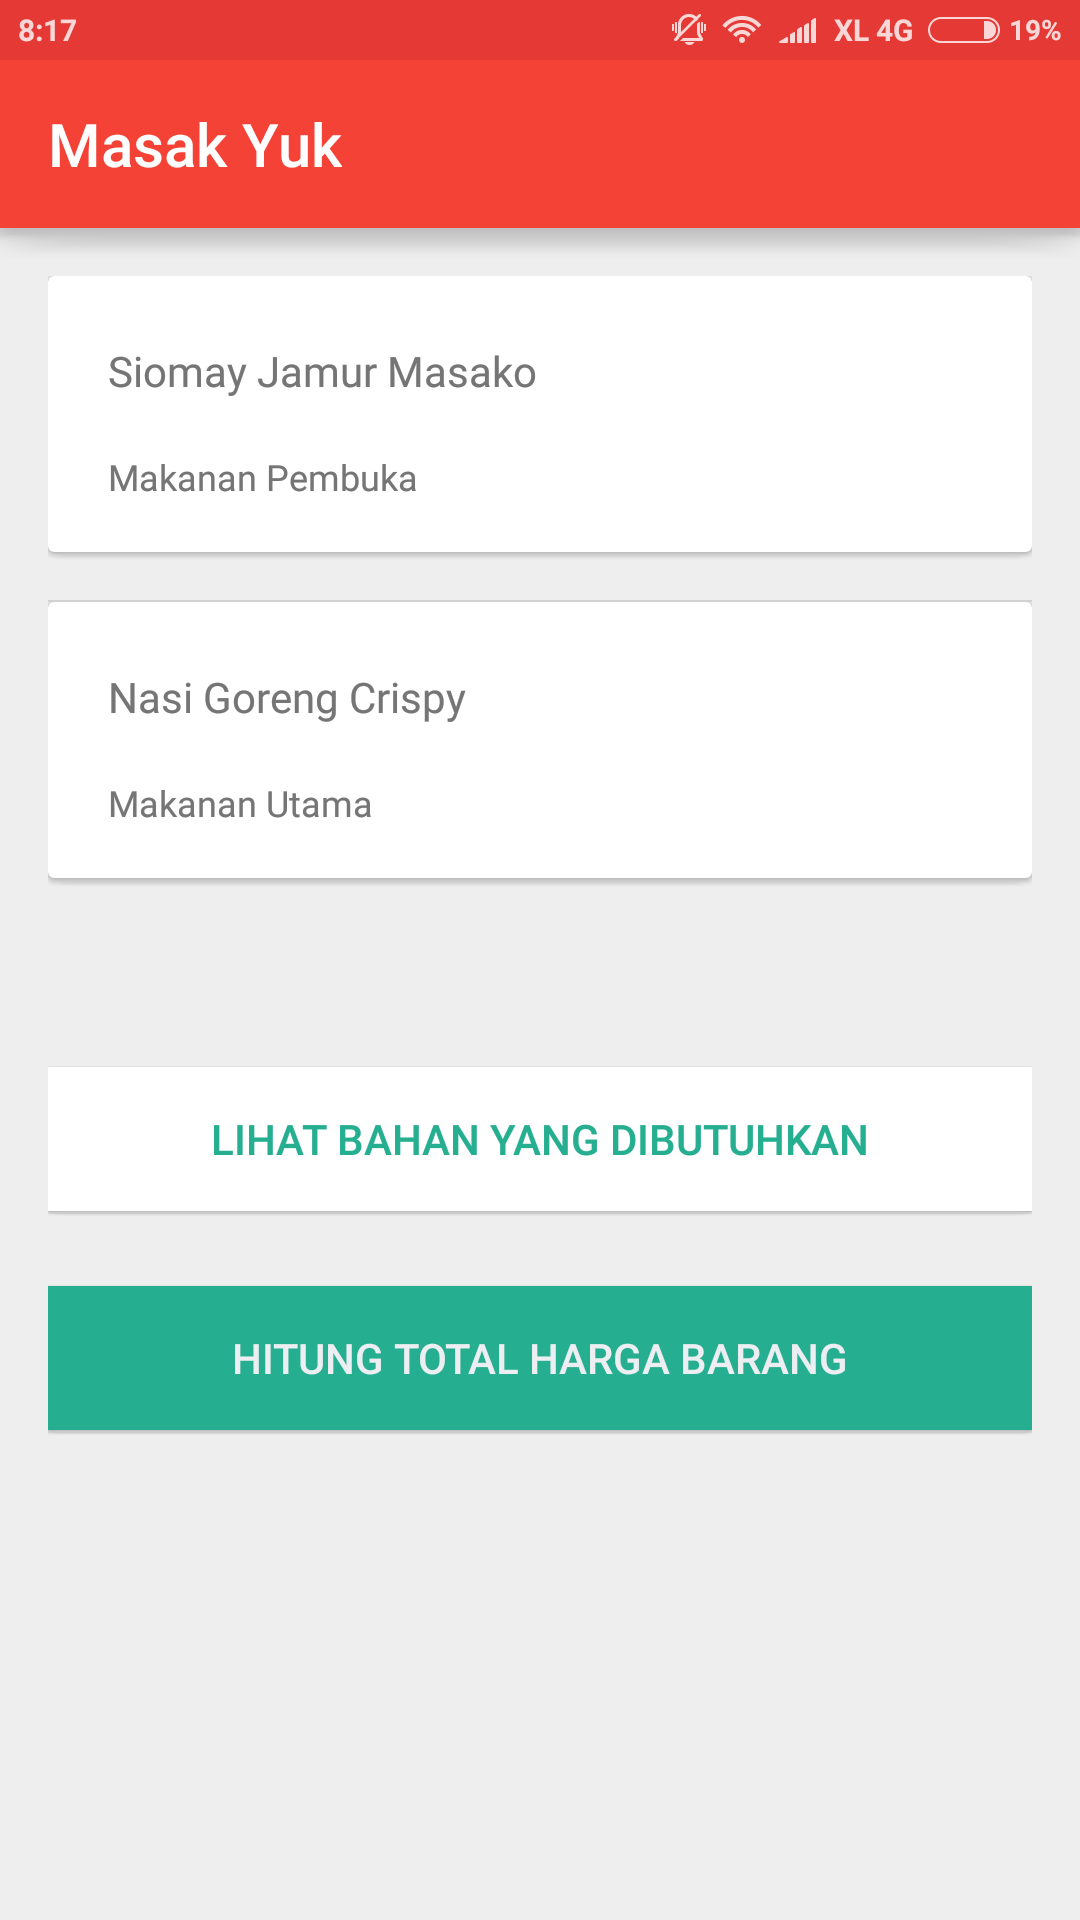
\includegraphics[width=0.3\textwidth]{gambar/mock-up/wishlist}
			\caption{\textit{Wishlist}}
		\end{figure}
		\begin{figure}[H]
			\centering
			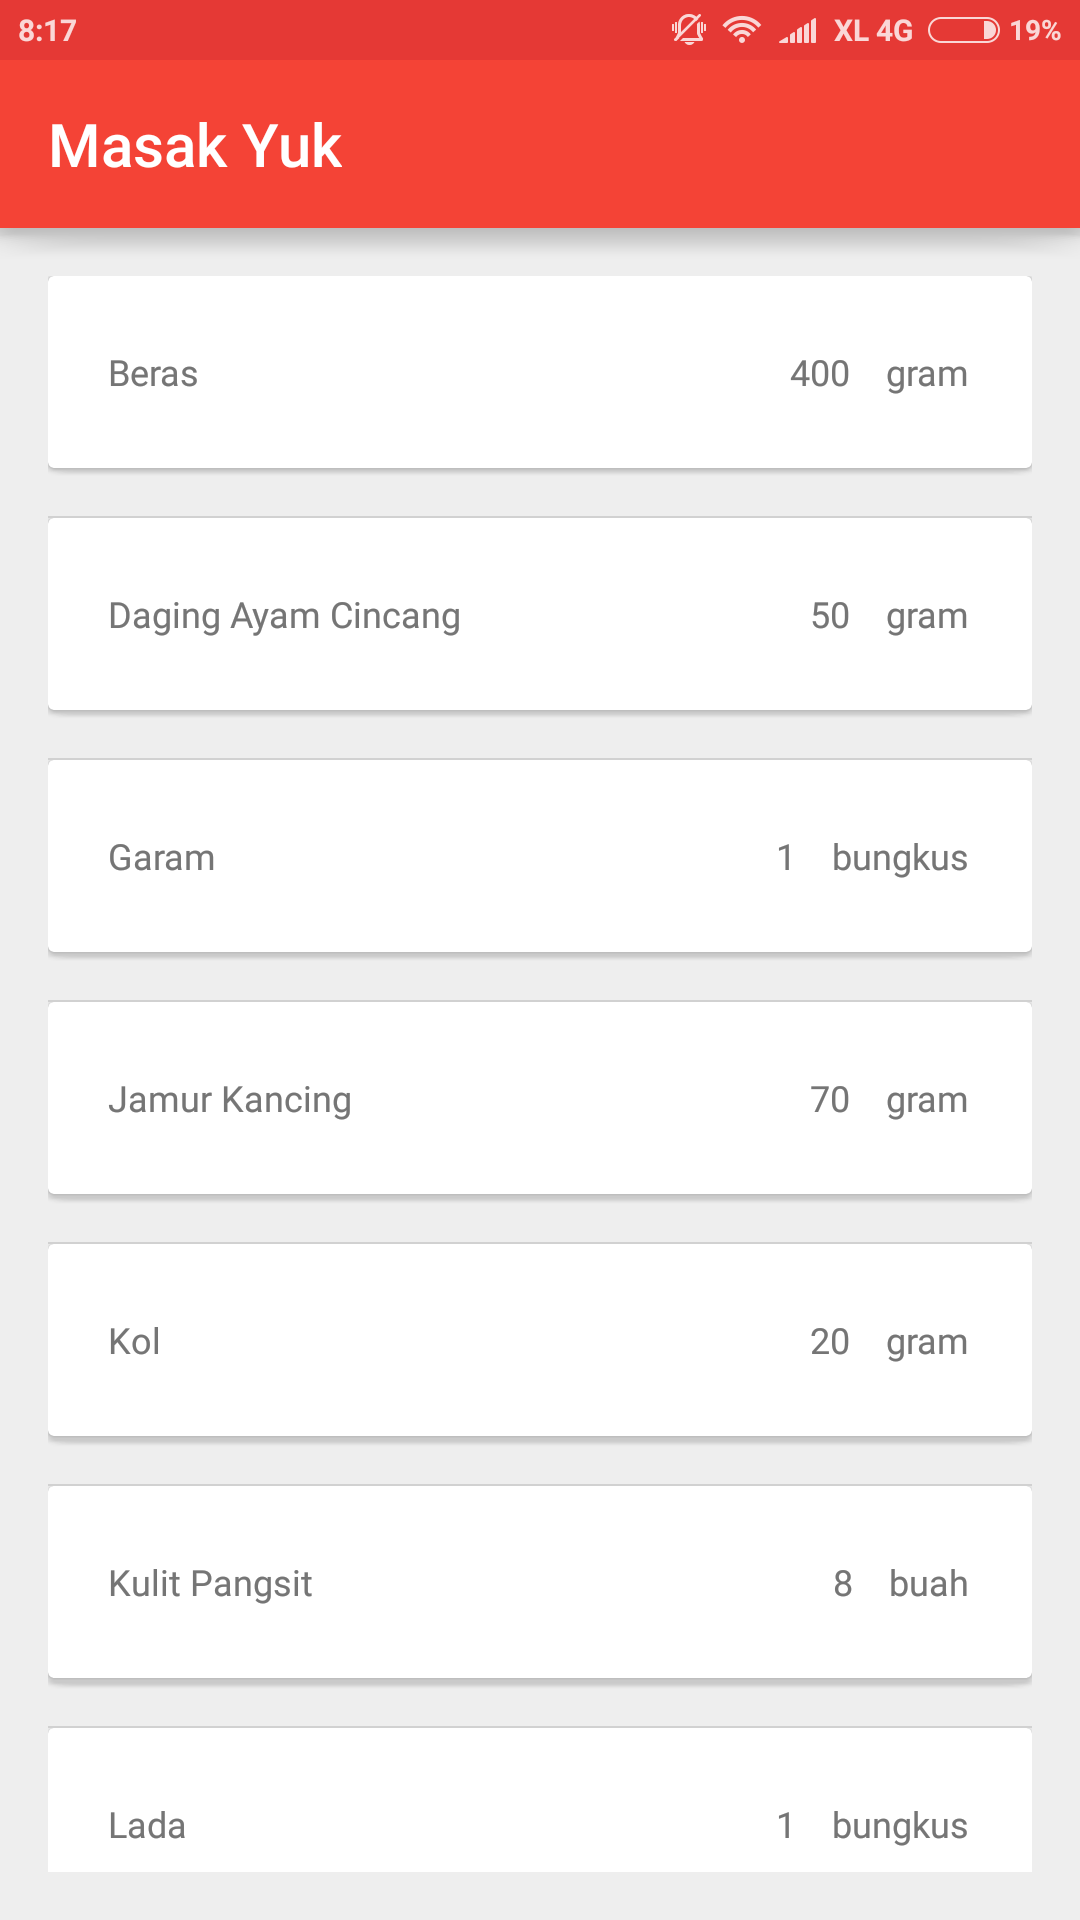
\includegraphics[width=0.3\textwidth]{gambar/mock-up/total_bahan}
			\caption{Total Bahan}
		\end{figure}	
		\begin{figure}[H]
			\centering
			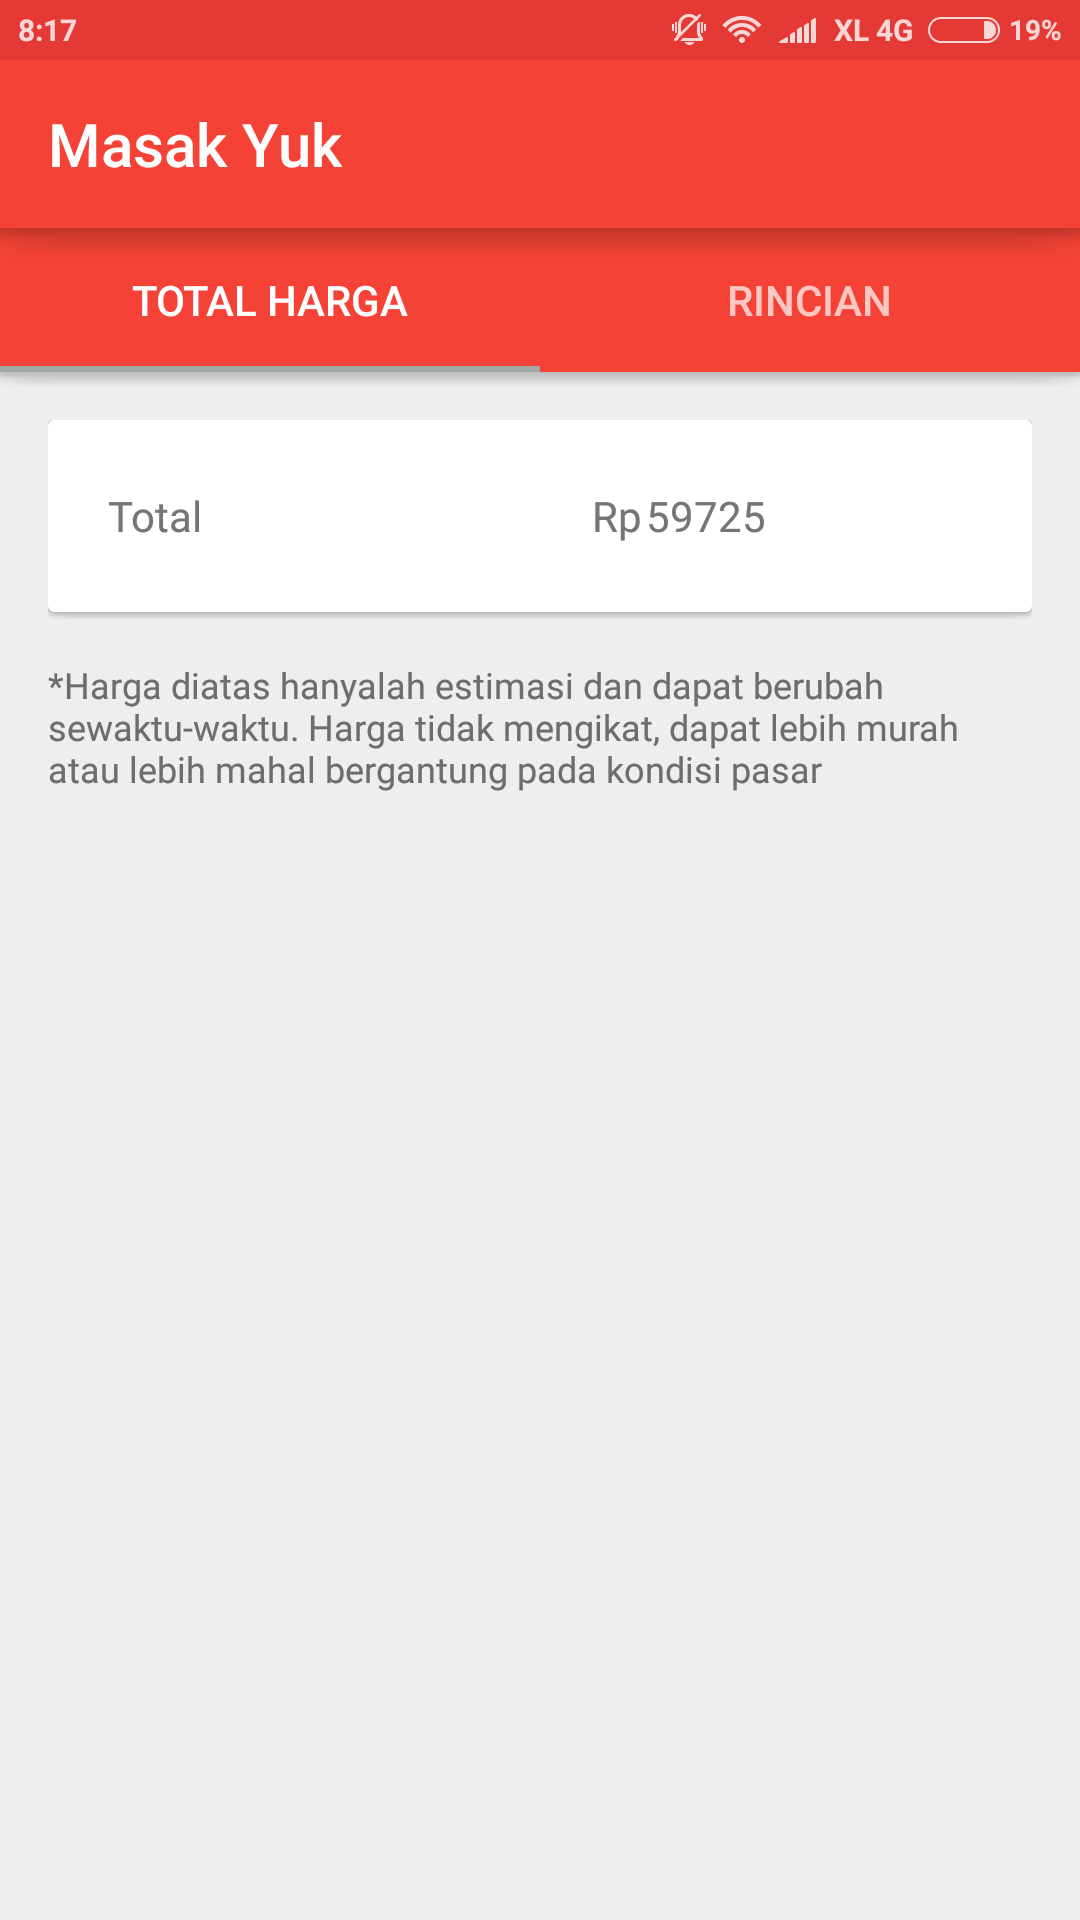
\includegraphics[width=0.3\textwidth]{gambar/mock-up/total_harga}
			\caption{Total Harga}
		\end{figure}	
		\begin{figure}[H]
			\centering
			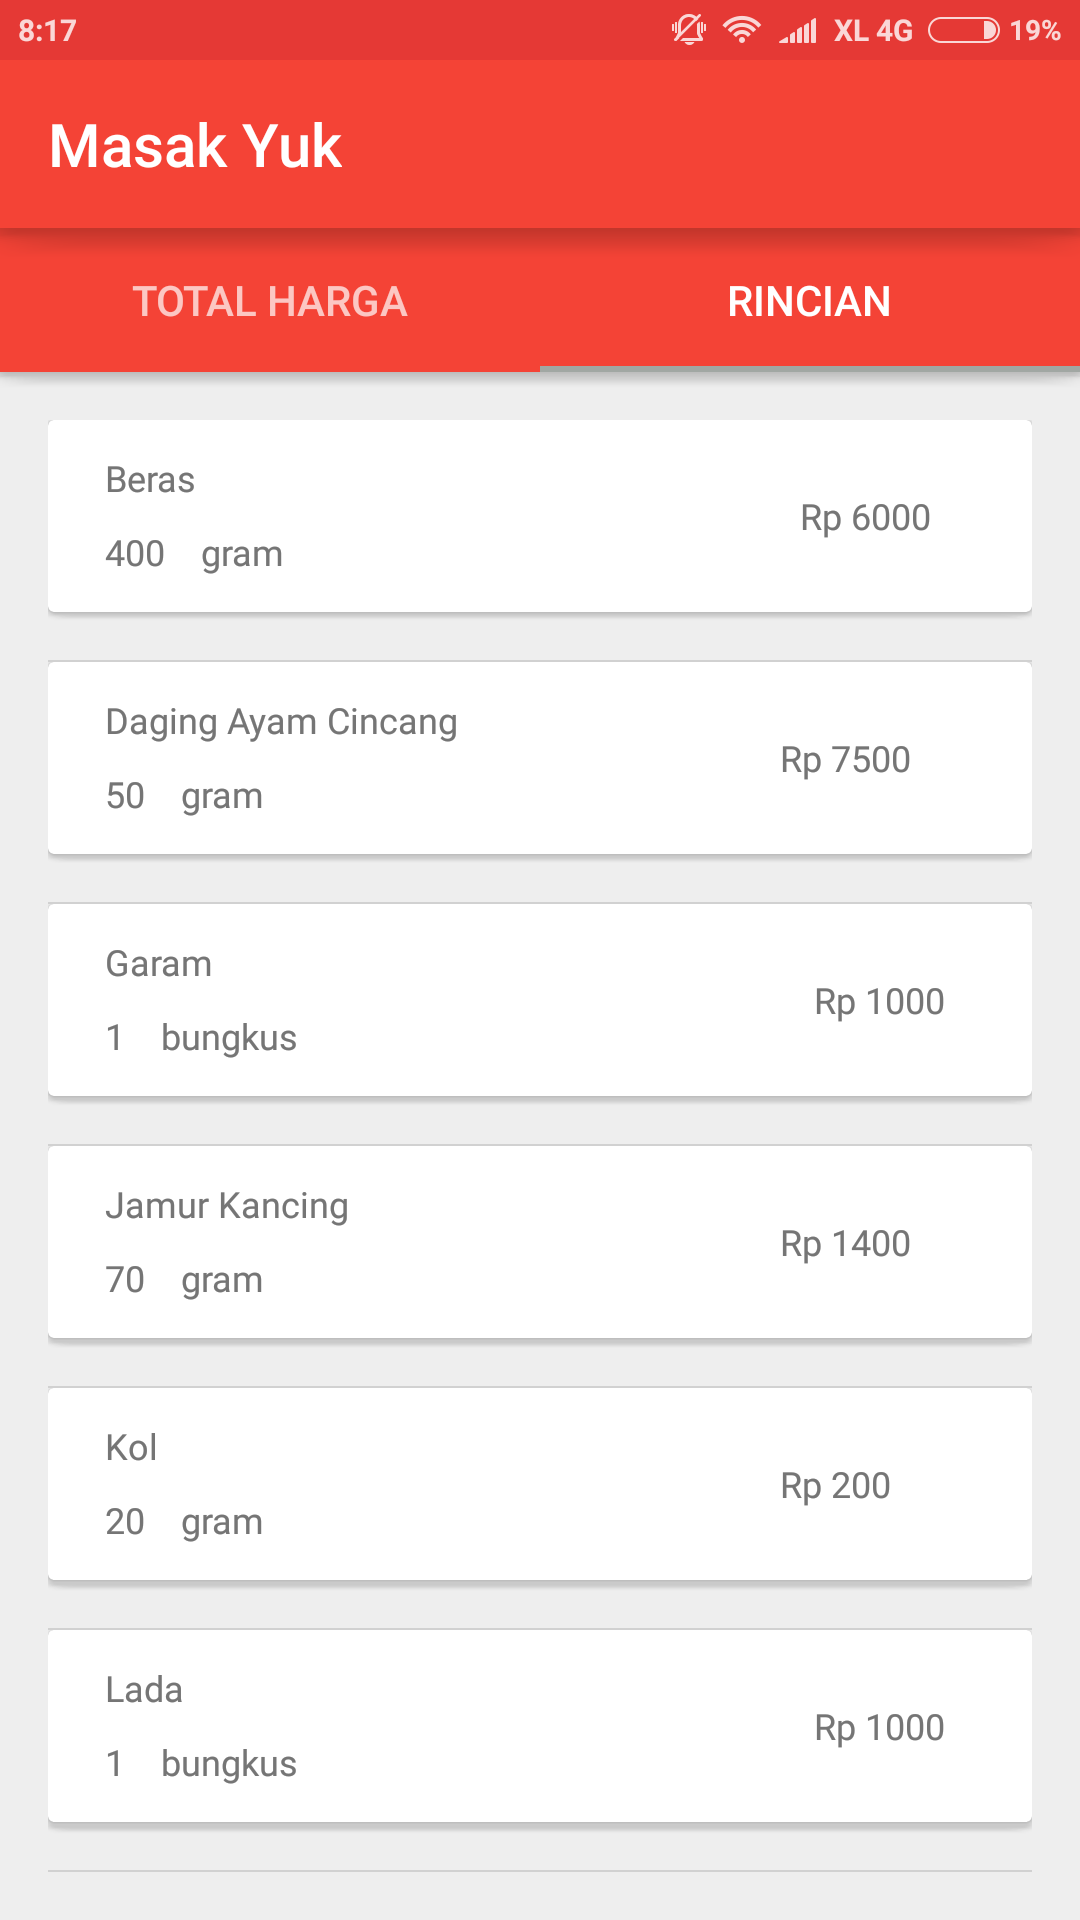
\includegraphics[width=0.3\textwidth]{gambar/mock-up/total_list_harga}
			\caption{Rincian Total Harga}
		\end{figure}	
		\begin{figure}[H]
			\centering
			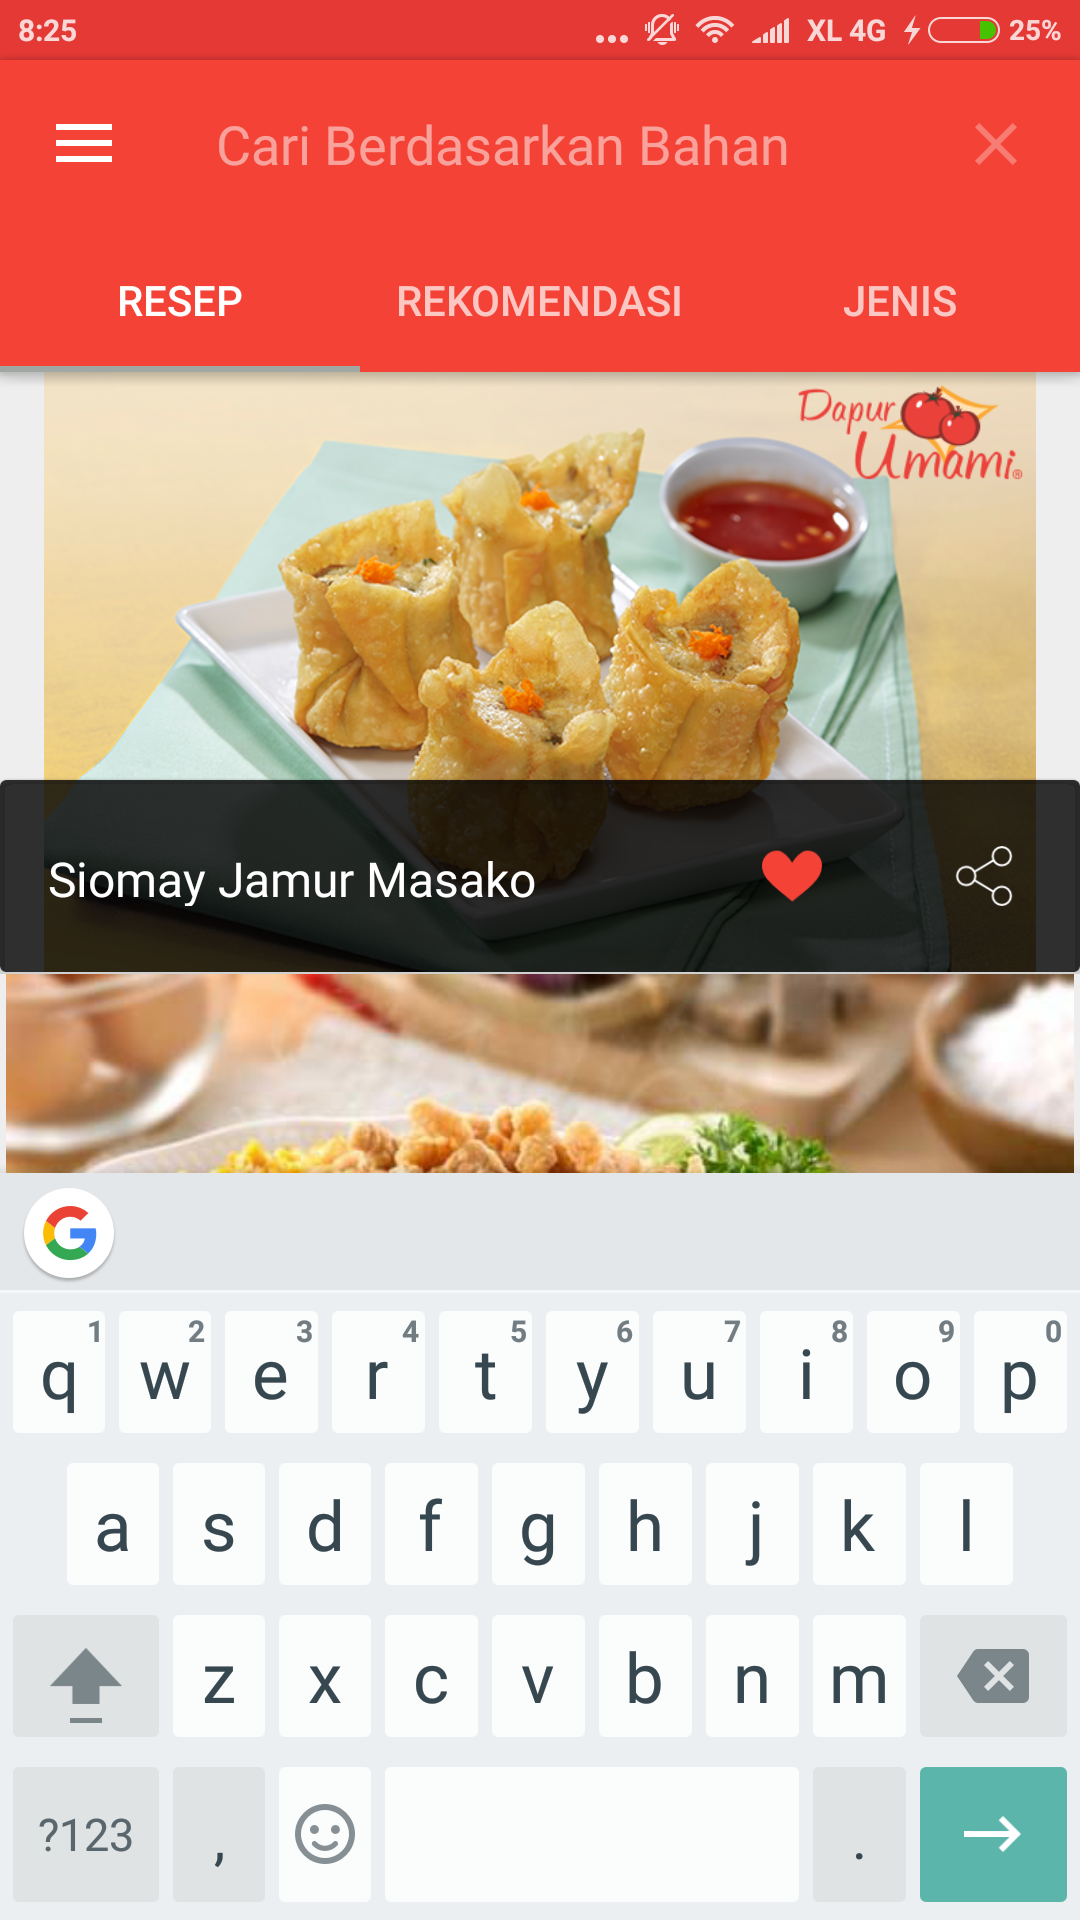
\includegraphics[width=0.3\textwidth]{gambar/mock-up/cari_bahan}
			\caption{\textit{Tab} Pencarian}
		\end{figure}								
		\begin{figure}[H]
			\centering
			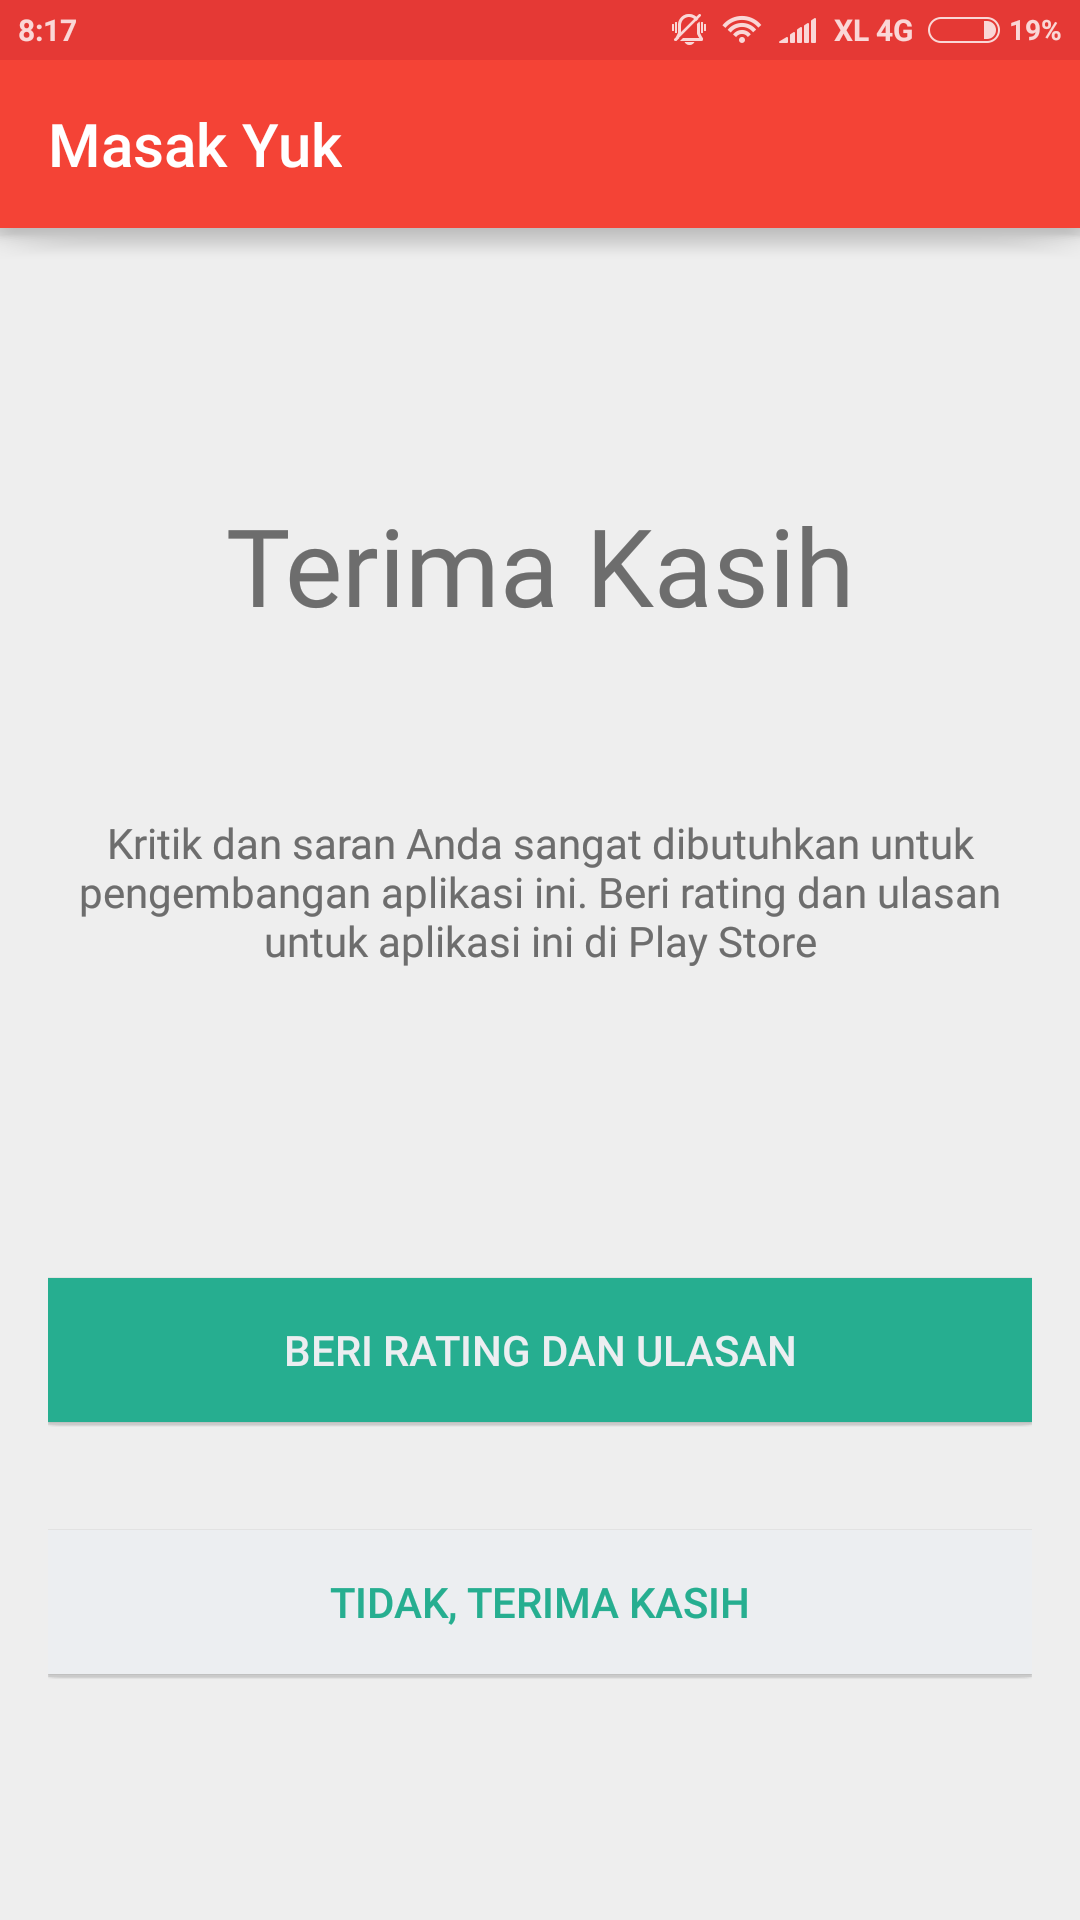
\includegraphics[width=0.3\textwidth]{gambar/mock-up/masukan}
			\caption{Laman Beri Masukan atau \textit{Feedback}}
			\label{mock-feedback}
		\end{figure}
				
\section{Konstruksi dan Pembangunan}
	Tahapan-tahapan dalam proses konstruksi dan pembangunan aplikasi berbasis resep masakan ini adalah sebagai berikut:
	\begin{enumerate}
		\item Membuat Basis Data
		\item Membuat API untuk Mengakses Basis Data
		\item Melakukan Input Data ke Basis Data
		\item Implementasi Desain Aplikasi
		\item Implementasi Metode Pertukaran Data antara Aplikasi dengan Basis Data
		\item Mengintegrasikan YouTube dengan Aplikasi Android
		\item Mengimplementasi Fitur Lainnya 
	\end{enumerate}

	\subsection{Membuat Basis Data}
		Basis data dibuat dengan menggunakan Basis Data MySQL atau MariaDB. Untuk mempercepat proses pengerjaan, penulis menggunakan aplikasi phpMyAdmin dalam membuat basis data secara keseluruhan, termasuk tabel dan entitas-entitas serta relasi yang terdapat di dalamnya. Basis data dibuat sesuai dengan ERD yang telah dibuat pada tahap desain.
		\begin{figure}[H]
			\centering
			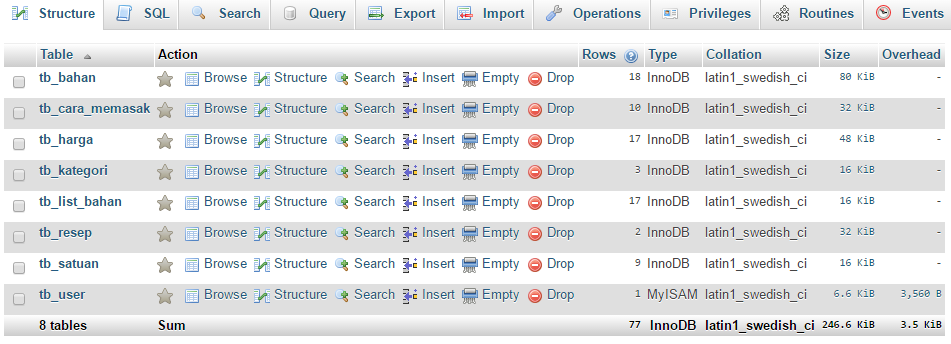
\includegraphics[width=1\textwidth]{gambar/phpmyadmin_masakyuk}
			\caption{Basis Data yang Dibuat dengan phpMyAdmin}
			\label{phpmyadmin}
		\end{figure}
	
	\subsection{Membuat API untuk Mengakses Basis Data}
		Untuk dapat mengakses data yang terdapat pada basis data, dimana data tersebut tersimpan dalam server dengan jenis basis data MySQL atau MariaDB, maka penulis perlu membuat kumpulan API. Pengguna membuat API dengan menggunakan \textit{php framework} yaitu CodeIgniter. CodeIgniter mengimplementasi arsitektur Model-View-Controller dimana semua perintah menuju database secara langsung disimpan dalam Model dan mengolah data yang didapatkan oleh Model dengan menggunakan Controller. Data yang sudah dioleh kemudian ditampilkan melalui View.
		\begin{figure}[H]
			\centering
			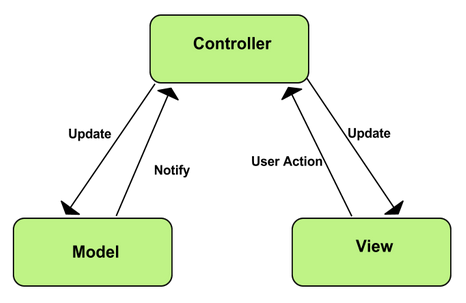
\includegraphics[width=0.8\textwidth]{gambar/mvc-arch}
			\caption{Bagan Alur Kerja MVC}
			\label{mvc-3}
		\end{figure}
		Namun untuk membuat API, penulis tidak menggunakan View dari CodeIgniter tersebut. Penulis hanya pelu menyimpan \textit{query} basis data pada model dan API tersimpan dalam bagian Controller. Aplikasi Android nantinya akan mengakses Controller tersebut dan dijadikan sebagai API untuk mendapatkan akses kepada basis data. API yang dibuat untuk Aplikasi Android hanya memiliki metode yang bersifat \textit{read only}. Data akan diterima oleh aplikasi dalam bentuk JSON (JavaScript Object Notation).
		\begin{figure}[H]
			\centering
			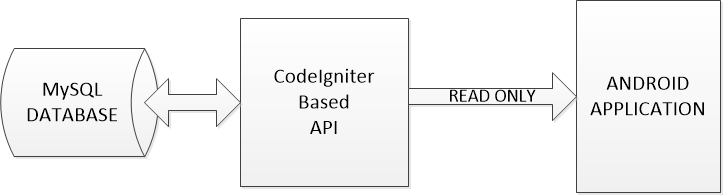
\includegraphics[width=1\textwidth]{gambar/api/codeigniter_based_api}
			\caption{Bagan Alur Kerja CodeIgniter-Based API}
			\label{ci_based_api}
		\end{figure}
		Sampel kode dari CodeIgniter-Based API yang telah dibuat oleh Penulis dapat dilihat pada Gambar \ref{ci_sample_api} atau pada Lampiran C dan D.
		\begin{figure}[H]
			\centering
			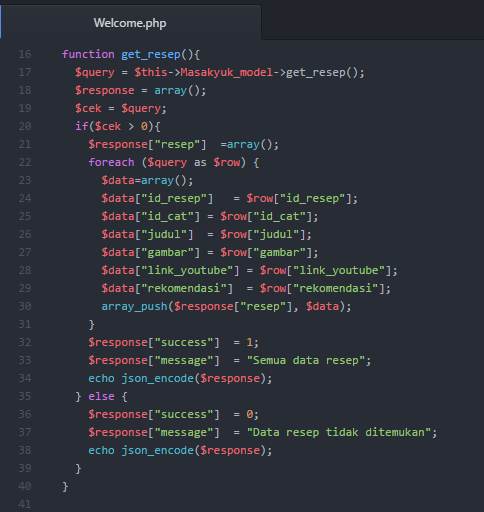
\includegraphics[width=1\textwidth]{gambar/sample-api-ci}
			\caption{Sampel Kode CodeIgniter API-Based yang Dibuat Penulis}
			\label{ci_sample_api}
		\end{figure}
	
	\subsection{Melakukan Input Data ke Basis Data}
		Input data ke dalam \textit{database} dapat dilakukan dengan dua cara, yaitu memasukkan data melalui phpMyAdmin atau memasukan data melalui aplikasi web khusus untuk memasukkan data ke dalam basis data.
		\begin{figure}[H]
			\centering
			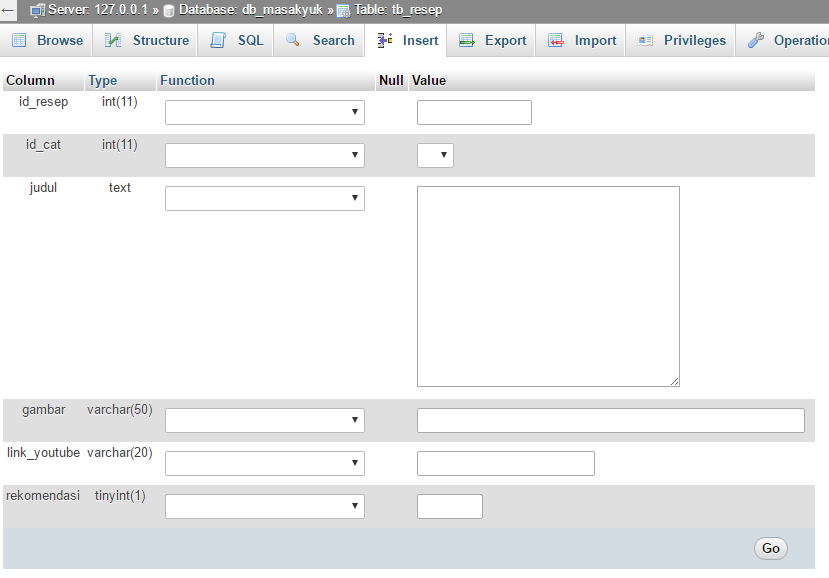
\includegraphics[width=1\textwidth]{gambar/insert-phpmyadmin}
			\caption{Input Data dengan phpMyAdmin}
			\label{insert_phpmyadmin}
		\end{figure} 
		Penulis mengembangkan aplikasi berbasis web dengan menggunakan \textit{framework} CodeIgniter yang khusus untuk memasukkan data ke dalam basis data. Adanya aplikasi berbasis web tersebut memudahkan penulis dalam memasukkan data-data ke dalam basis data, mulai dari data resep, bahan, hingga data harga bahan.
		\begin{figure}[H]
			\centering
			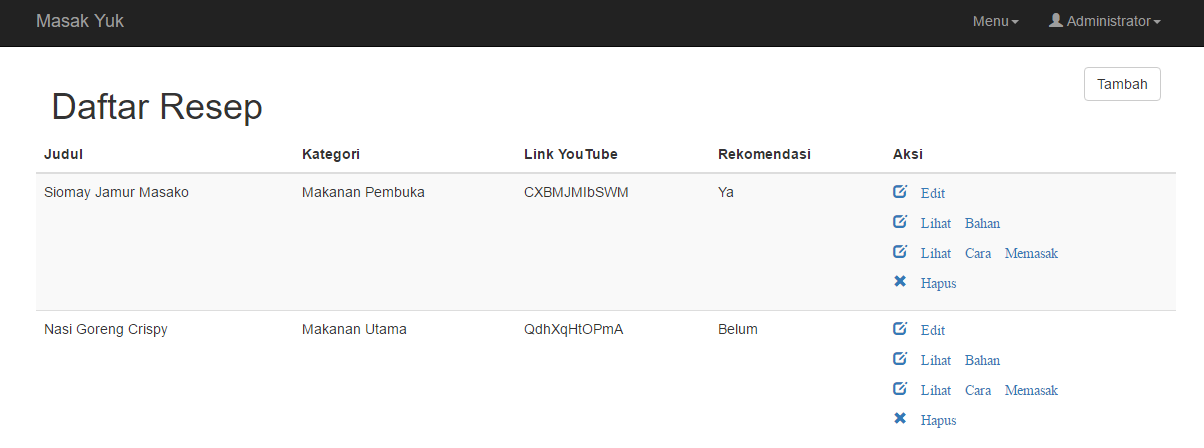
\includegraphics[width=1\textwidth]{gambar/web-list-resep}
			\caption{Tampilan List Resep pada Aplikasi Berbasis Web}
			\label{web-list-resep}
		\end{figure} 
		\begin{figure}[H]
			\centering
			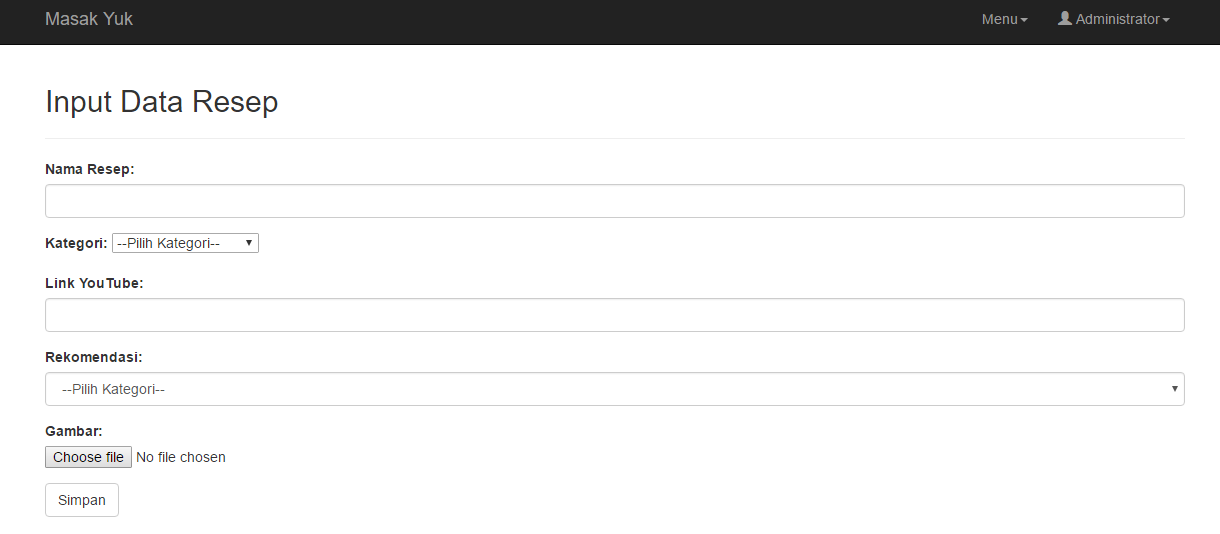
\includegraphics[width=1\textwidth]{gambar/web-input-resep}
			\caption{Tampilan Input Resep pada Aplikasi Berbasis Web}
			\label{web-input-resep}
		\end{figure} 		
		Penulis melakukan sedikit modifikasi pada API yang telah dibuat dengan mengubah metode \textit{read only} menjadi \textit{read and write} dengan catatan yaitu write hanya diperbolehkan pada aplikasi berbasis web yang digunakan untuk memasukkan data-data yang dibutuhkan.  
		\begin{figure}[H]
			\centering
			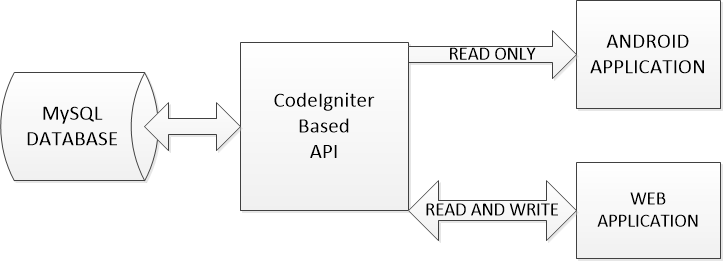
\includegraphics[width=1\textwidth]{gambar/api/ci-api-web-chart}
			\caption{Bagan Alur Kerja CodeIgniter-Based API Hasil Modifikasi}
			\label{web-modification-resep}
		\end{figure} 	
	
	\subsection{Implementasi Desain Aplikasi}
		Desain Aplikasi sudah diimplementasikan kedalam bentuk \textit{layout} Android Studio yaitu dengan format xml sehingga penulis dapat melewati tahap implementasi desain ini. Implementasi dapat dilihat pada Bagian 3.2.6.
		
	\subsection{Implementasi Metode Pertukaran Data antara Aplikasi dengan Basis Data}
		Pada tahap ini, penulis mencoba mengimplementasikan API yang telah dibuat ke dalam aplikasi Android. Hal itu dilakukan agar aplikasi dapat melakukan pertukaran data dengan basis data dengan dijembatani oleh API yang telah dibuat sebelumnya. Pada aplikasi berbasis web, pertukaran data dilakukan dengan memanfaatkan Form GET/POST seperti pada Gambar \ref{req-html}.
		\begin{figure}[H]
			\centering
			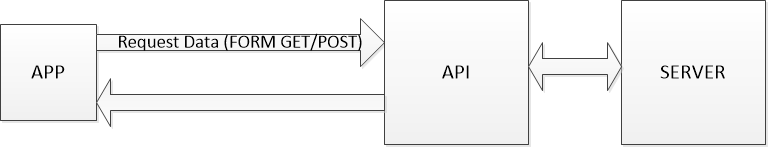
\includegraphics[width=1\textwidth]{gambar/new/req_html}
			\caption{Bagan Alur Kerja Form GET/POST}
			\label{req-html}
		\end{figure}
		Dalam pengembangan aplikasi Android, salah satu cara untuk dapat memanggil CodeIgniter-Based API yang telah dibuat adalah dengan menggunakan Volley. Android Volley Library adalah sebuah \textit{library} yang disediakan oleh Google untuk dapat memfasilitasi akses \textit{Web-Based} API pada aplikasi Android sebagai media pertukaran data antara aplikasi dengan basis data. Cara Kerja Volley secara umum menyerupai Form GET/POST pada aplikasi berbasis web.
		\begin{figure}[H]
			\centering
			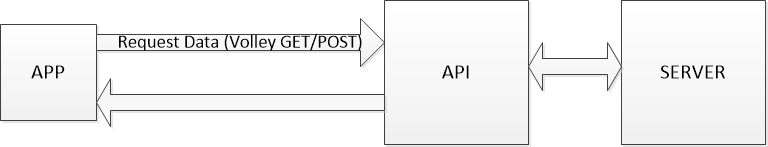
\includegraphics[width=1\textwidth]{gambar/new/req_volley}
			\caption{Bagan Alur Kerja Volley}
			\label{req-volley}
		\end{figure}
		Untuk dapat menggunakan Volley, penulis harus terlebih dahulu menambahkan compile 'com.android.volley:volley:1.0.0' pada berkas build.gradle yang terdapat di dalam direktori app.    	
	\subsection{Mengintegrasikan YouTube dengan Aplikasi Android}
		 Untuk dapat memainkan video YouTube pada aplikasi Android, maka dibutuhkan YouTube Android Player API sebagai perantara aplikasi dengan basis data YouTube. Penulis melakukan sedikit modifikasi pada implementasi YouTube Android Player API karena penggunaan Fragment pada Resep Activity. Ketika suatu \textit{class} pada Java Android Studio menggunakan Fragment, maka diperlukan \textit{class} yang melakukan ekstensi (\textit{extends}) dengan AppCompatActivity untuk mendukung pengelolaan beberapa Fragment yang akan ditampilkan pada sebuah Activity. Sedangkan YouTube Android Player API mewajibkan penggunanya untuk melakukan ekstensi terhadap \textit{class} YouTubeBaseActivity
 		\begin{figure}[H]
		 	\centering
		 	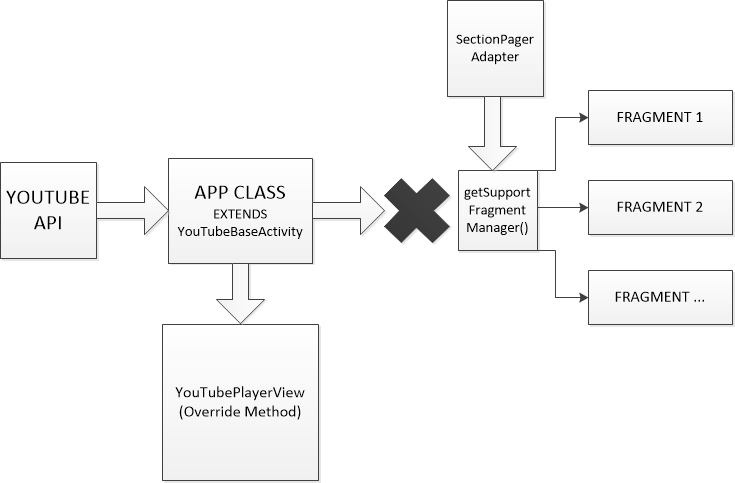
\includegraphics[width=1\textwidth]{gambar/new/youtube_player_view}
		 	\caption{Bagan Alur Kerja YouTubePlayerView pada sebuah Activity}
		 	\label{youtube-player-view}
		 \end{figure}
		\vspace{1cm}
		Apabila Activity tetap mengekstensi YouTubeBaseActivity, maka Activity tersebut tidak dapat mengelola Fragment yang terdapat didalamnya karena kehilangan metode getSupportFragmentManager() yang berasal dari ekstensi \textit{class} terhadap AppCompatActivity. Maka dari itu, penulis melakukan modifikasi dengan tidak menggunakan YouTubePlayerView, melainkan menggunakan YouTubePlayerFragment. Keputusan tersebut diambil karena YouTubePlayerFragment "lebih ramah" terhadap Activity yang memiliki Fragment dengan tidak perlu mengekstensi \textit{class} YouTubeBaseActivity sehingga seluruh Fragment yang ada pada sebuah Activity dapat dikelola dengan baik. Perbedaannya adalah seluruh metode yang diberikan oleh YouTube Android Player API tidak dilakukan \textit{override}, melainkan langsung diinisialisasikan pada metode onCreate sebuah Activity. 
 		\begin{figure}[H]
			\centering
			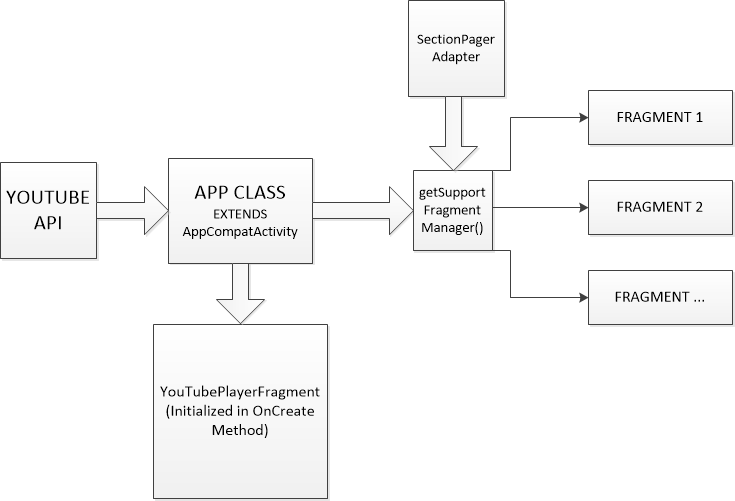
\includegraphics[width=1\textwidth]{gambar/new/youtube_player_fragment}
			\caption{Bagan Alur Kerja YouTubePlayerFragment pada sebuah Activity}
			\label{youtube-player-frag}
		\end{figure}
		\vspace{1cm}
		Sampel kode implementasi YouTubePlayerFragment terdapat pada Gambar \ref{youtube-frag-sampel}.
 		\begin{figure}[H]
			\centering
			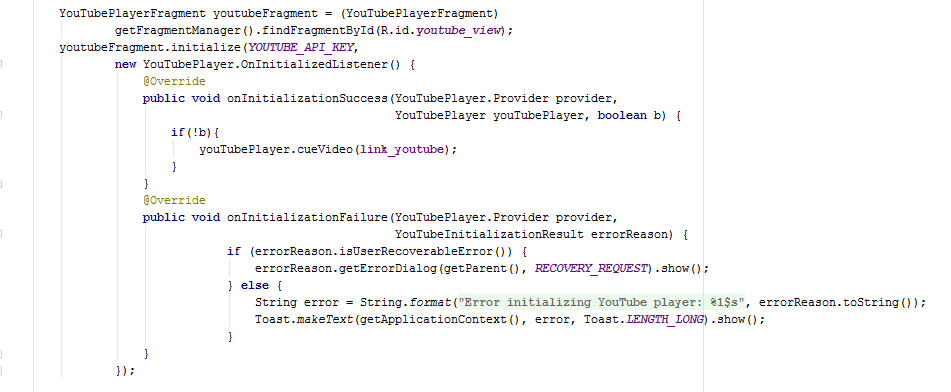
\includegraphics[width=1\textwidth]{gambar/new/youtube_fragment}
			\caption{Sampel Kode Implementasi YouTubePlayerFragment pada Metode onCreate sebuah Activity}
			\label{youtube-frag-sampel}
		\end{figure}
	\subsection{Mengimplementasi Fitur Lainnya}
		Fitur lain yang diimplementasikan oleh penulis adalah fitur penyimpanan \textit{wishlist}, menghitung total bahan pada resep yang terdapat dalam \textit{wishlist}, menghitung total harga bahan yang terdapat pada \textit{wishlist} dan menampilkan rincian harga per bahan. \textit{Wishlist} sendiri dibuat dengan memanfaatkan basis data SQLite dengan menggunakan bahasa query yang sama yakni SQL. Basis data SQLite bersifat lokal dan terdapat didalam aplikasi itu sendiri. Jadi, apabila pengguna aplikasi menghapus data aplikasi pada ponselnya, maka data \textit{wishlist} pun juga akan hilang.
		
		Wishlist mampu menampung maksimal tiga resep masakan. Untuk dapat menghitung total bahan dan total harga bahan yang terdapat pada resep-resep tersebut, maka data yang terdapat di dalam SQLite dikirimkan dan diolah oleh API yang telah dibuat untuk kemudian disalurkan kembali hasil perhitungannya pada aplikasi. Alur dari proses penyimpanan pada \textit{wishlist} hingga perhitungan total bahan dan harga bahan dijelaskan pada Gambar \ref{fitur-lain}
		\begin{figure}[H]
			\centering
			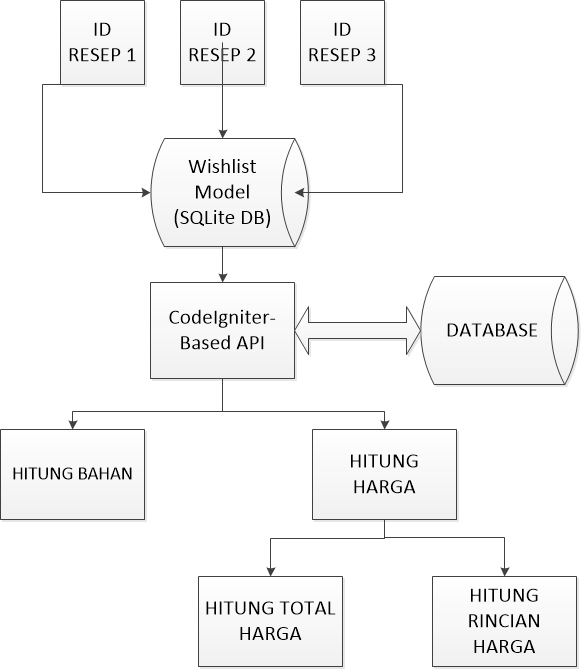
\includegraphics[width=1\textwidth]{gambar/new/fitur_lain}
			\caption{Alur Penyimpanan pada SQLite dan Pengolahan Total Bahan dan Harga Bahan}
			\label{fitur-lain}
		\end{figure}